%%%%%%%%%%%%%%%%%%%%%%%%%%%%%%%%%%%%%%%%%%%%%%%%%%%%%%%
%% Bachelor's & Master's Thesis Template             %%
%% Copyleft by Artur M. Brodzki & Piotr Woźniak      %%
%% Faculty of Electronics and Information Technology %%
%% Warsaw University of Technology, 2019-2020        %%
%%%%%%%%%%%%%%%%%%%%%%%%%%%%%%%%%%%%%%%%%%%%%%%%%%%%%%%

\documentclass[
    left=2.5cm,         % Sadly, generic margin parameter
    right=2.5cm,        % doesnt't work, as it is
    top=2.5cm,          % superseded by more specific
    bottom=3cm,         % left...bottom parameters.
    bindingoffset=6mm,  % Optional binding offset.
    nohyphenation=false % You may turn off hyphenation, if don't like.
]{eiti/eiti-thesis}
\langpol % Dla języka angielskiego mamy \langeng
\graphicspath{{img/}}             % Katalog z obrazkami.
\addbibresource{bibliografia.bib} % Plik .bib z bibliografią

\begin{document}

%--------------------------------------
% Strona tytułowa
%--------------------------------------
\MasterThesis % Dla pracy inżynierskiej mamy \EngineerThesis
\instytut{Informatyki}
\kierunek{Informatyka}
\specjalnosc{Inżynieria Systemów Informatycznych}
\title{
    Badanie nierzetelnych informacji w mediach społecznościowych\\ i ich automatyczna klasyfikacja na podstawie kontekstu
}
\engtitle{ % Tytuł po angielsku do angielskiego streszczenia
    Analysis of fake news in social media and their automatized\\ context-based classification
}
\author{Sylwia Genowefa Pytko}
\album{296179}
\promotor{prof. Piotr Gawrysiak}
\date{\the\year}
\maketitle

%--------------------------------------
% Streszczenie po polsku
%--------------------------------------
\cleardoublepage % Zaczynamy od nieparzystej strony
\streszczenie W ostatnich latach rozprzestrzenianie się nierzetelnych informacji w mediach społecznościowych stało się poważnym problemem, jednak nadal mało inicjatyw podejmuje się rozwiązania tego problemu w sposób automatyczny. W ramach niniejszej pracy zostały przedstawione czynniki sprzyjające rozprzestrzenianiu się nierzetelnych informacji w Internecie oraz zostały omówione sposoby rozpoznawania ich w sposób zarówno manualny jak i automatyczny. Głównym celem pracy jest analiza danych polskojęzycznych pobranych z platformy Twitter w celu wykrycia charakterystycznych właściwości nierzetelnych informacji oraz dokonanie badania automatycznej klasyfikacji postów w mediach społecznościowych na podstawie danych kontekstowych jakimi są użytkownicy je udostępniający. Wyniki przeprowadzonych badań w tej pracy pokazują obiecujące wyniki dalszego rozwoju automatycznego rozpoznawania informacji.
\slowakluczowe klasyfikacja, fałszywe informacje, dezinformacja

%--------------------------------------
% Streszczenie po angielsku
%--------------------------------------
\newpage
\abstract Last few years the spread of fake news in social media became a massive problem, however attempts to automatize the process of their classification are still scarce. This thesis consists of presenting factors that impact the spread of fake news on the Internet and analyses methods of discerning them, both manually and automatically. The main purpose of the thesis is an analysis of Polish language Twitter entries in order to detect defining characteristics of fake news and attempt to build an automatic classification system based on the context that takes the form of users spreading them. Results of the aforementioned study show a promise regarding possibilities of further development of automatic information recognition.
\keywords classification, fake news, disinformation

%--------------------------------------
% Oświadczenie o autorstwie
%--------------------------------------
\cleardoublepage  % Zaczynamy od nieparzystej strony
\pagestyle{plain}
\makeauthorship

%--------------------------------------
% Spis treści
%--------------------------------------
\cleardoublepage % Zaczynamy od nieparzystej strony
\tableofcontents

%--------------------------------------
% Rozdziały
%--------------------------------------
\cleardoublepage % Zaczynamy od nieparzystej strony
\pagestyle{headings}

\newpage % Rozdziały zaczynamy od nowej strony.
\section{Wstęp}
Kwestia wiarygodności informacji napływających do nas ze wszystkich mediów stała się ostatnio gorącym tematem. Mimo faktu, że problem występuje od zawsze, w\,ostatnich latach zwrócił na siebie dużo uwagi. Przy ilości informacji jaka jest udostępniana w Internecie, w\,szczególności dzięki możliwości udostępniania wszystkiego poprzez portale społecznościowe, szerzenie dezinformacji stało się bardzo proste i\,szybkie. Mogą one przyjmować rozmaitą formę zaczynając na krótkiej formie tekstowej jaką są Tweety, poprzez kłamliwe artykuły naukowe, przerobione zdjęcia na zmanipulowanych filmach wideo kończąc. Należy więc podjąć próbę wykrycia prawdziwości pojawiających się treści. Można to wykonać przez pracę człowieka lub automatycznie.
\par
W ostatnich latach powstaje coraz więcej inicjatyw próbujących zrozumieć i\,powstrzy- mać to zjawisko skupiając się zarówno na podłożu socjologicznym jak również tworząc nowe rozwiązania informatyczne których zadaniem będzie pomoc użytkownikom w\,rozróżnieniu prawdy od dezinformacji. Takich projektów jednak jest nadal bardzo mało i\,w\,większości nie obejmują one innych języków niż angielski.
\par
W poniższej pracy przedstawiono opis problemu jakim są nierzetelne informacje oraz zebrano dotychczasowe rozwiązania oceny prawdziwości treści. Następnie opracowano badania porównujące cechy kont oraz publikowanych treści w\,mediach społecznościowych. Badano treści w\,języku polskim oraz porównywano konta zakwalifikowane jako nierzetelne do kont określanych jako wiarygodne. Takiego podziału dokonano na podstawie kilku niezależnych źródeł. Na podstawie zebranych danych dokonano badania automatycznej klasyfikacji treści pochodzących z\,portalu społecznościowego na podstawie ich kontekstu. Klasyfikowano czy post należy do klasy nierzetelnych czy też nie wykorzystując wiedzę jego odbiorcach.
\par
Na wstępie przeprowadzono rozpoznanie problemu, czynniki mu sprzyjające oraz jego wpływ na rzeczywistość. Następnie na podstawie dostępnej literatury i\,istniejących badań przedstawiono najbardziej popularne sposoby rozwiązania problemu klasyfikacji informacji pod względem ich wiarygodności. 
\par
Okazuje się, że większość istniejących projektów w\,tym temacie skupia się wyłącznie na tematyce polityki w\,USA. Jedynie pojedyncze zespoły podjęły do tej pory działania obejmujące obszary związane z\,innymi językami niż angielski oraz inną strefą tematyczną. Według najlepszej wiedzy autora, nie istnieją w\,tym momencie żadne inicjatywy podejmujące temat klasyfikacji informacji w\,mediach społecznościowych w\,języku polskim. Z tego powodu poniższa praca w\,dalszej swojej części skupia się na rozpoznaniu problemu wiarygodności informacji w\,polskiej przestrzeni internetowej. Przytoczone zostaną badania opinii społecznej oraz zanalizowane zostaną dostępne badania obejmujące tematy Unii Europejskiej. 
\par
W drugiej części pracy zostanie przeprowadzona oraz opisana analiza wybranych danych pochodzących z\,polskojęzycznych postów opublikowanych w mediach społecznościowych. Celem tej analizy będzie znalezienie właściwości i\,charakterystyk kont uznanych za nierzetelne. W\,celu analizy porównawczej konta te zostaną przeciwstawione kontom należącym do profesjonalnych serwisów informacyjnych, serwisów o dużej liczbie odsłon oraz portali specjalizujących w sprawdzaniu prawdziwości innych mediów (tzw.\,factchecking).
\par
Ostatnim badaniem przeprowadzonym w\,ramach tej pracy będzie dokonanie próby automatycznej klasyfikacji treści pochodzących z\,mediów społecznościowych na podstawie ich kontekstu. Kontekstem, który zostanie przyjęty będzie interakcja użytkowników portalu z\,badanymi treściami. Celem tego badania jest sprawdzenie możliwości wykonania takiej klasyfikacji i\,jej precyzji. Dodatkowo zostanie zbadane jak duża musi być zaklasyfikowana próbka treningowa, aby otrzymać zadowalające wyniki klasyfikacji. Do wykonania tej klasyfikacji zostaną użyte dwa algorytmy. Pierwszym z\,nich jest klasyczny algorytm uczenia maszynowego jakim jest regresja logistyczna, a\,drugim będzie zastosowanie algorytmu etykietowania przez użytkowników używając właściwości rozprzestrzeniania wiedzy w\,sieci. 
\par
Na koniec podsumowana zostanie cała zdobyta wiedza oraz wyniki przeprowadzonych badań. Zostaną zebrane wnioski oraz wynikająca z\,nich nauka dla przyszłych inicjatyw chcących badać lub automatycznie wykrywać nieprawdziwe informacje publikowane za pomocą mediów społecznościowych. 

  

\newpage % Rozdziały zaczynamy od nowej strony.
\section{Podjęta problematyka}
Zjawisko intencjonalnego publikowania nieprawdziwych informacji dostało nazwę fake news. 
Ten neologizm został również zaadoptowany w\,języku polskim. Słownik języka polskiego PWN w\,dziale ciekawostki definiuje zwrot fake news jako „nieprawdziwe, fałszywe wiadomości, najczęściej rozpowszechniane przez tabloidy w\,celu wywołania sensacji, bądź zniesławienia kogoś (najczęściej polityka)”. Według językoznawcy nie jest to w\,języku polskim już tylko słowo slangowe, jako że wygrało w\,plebiscycie słowników Collinsa w\,roku 2017\footnote{\url{https://sjp.pwn.pl/ciekawostki/haslo/fake-news;6368870.html}}.  Inaczej możemy to zjawisko nazywać dezinformacją, które jest definiowana jako „fałszywa, rzekoma informacja, zamierzone wprowadzenie w\,błąd” \footnote{\url{https://sjp.pl/dezinformacja}}. 
Może ono objawiać się pod różnymi formami, najbardziej kojarzą się z\,ich pierwotną formą jaką są artykuły w\,mediach szerzące nieprawdę. Mimo że ten problem występuje tak długo jak istnieją media obecnie jednak jego wpływ jest dużo większy. 

\subsection{Problematyka nierzetelnych informacji}
Szerzenie się nieprawdziwych, nierzetelnych informacji w\,mediach, z\,których pobieramy wiedzę o świecie nie może być ignorowane. Wielkość tego zjawiska już teraz stwarza dużo problemów i \,ciągle się powiększa. Coraz więcej osób pobiera najświeższe informacje o wydarzeniach z\,internetu. Informacje można te podzielić ze względu na źródło z\,jakiego pochodzą. Mogą być one bowiem publikowane przez tradycyjne media znane z\,formy papierowej lub telewizyjnej posiadające własną stronę internetową. Ale internet daje również duże możliwości publikowania własnych treści wszystkim użytkownikom, dzieje się to głównie poprzez blogi i\,portale społecznościowe.  \par
Nierzetelne informacje w\,Internecie są poważnym problemem. 68\% Europejczyków natrafia na informacje, które zakłamują rzeczywistość przynajmniej raz w\,tygodniu a\,połowa z\,nich nawet codziennie \cite{Eurobarometer4642018}. Na szczęście 71\% z\,nich twierdzi, że jest raczej pewnych w\,swoich umiejętnościach wykrycia czy czytana przez nich informacja o wydarzeniach jest prawdziwa czy też nie. Mimo to nierzetelne informacje występują w\,mediach społecznościowych a\,użytkownicy często wchodzą z\,nimi w\,interakcje poprzez udostępnianie ich dalej.
\par Mimo tego, że więcej użytkowników Internetu nadal bardziej ufa źródłom związanym z\,tradycyjnymi mediami niż informacjom generowanym przez użytkowników \cite{rieh2014credibility} to według badań z\,2018 roku 68 procent ankietowanych amerykanów zadeklarowało, że zdarza im się czytać informacje za pomocą portali społecznościowych \cite{PewNewsUse2018}. Takie badania co roku przeprowadza Centrum Badań Pew. Według ich danych wzrost liczby osób korzystających z\,portali społecznościowych do zdobywania wiadomości o świecie w\,ostatnim roku przystopowała po czasie dużego wzrostu w\,poprzednich latach.

\subsubsection{Social media}
Widać, więc jak duże jest nadal znaczenie portali społecznościowych w\,szerzeniu informacji. Dzieje się tak z\,kilku powodów. Dla użytkowników jest to po prostu wygodne. Przeglądając główną stronę aplikacji użytkownik dostaje posty subskrybowanych przez siebie stron informacyjnych lub posty z\,którymi weszli w\,interakcje jego znajomi. Dzieje się tak w\,szczególności dla portalu Facebook, gdzie większość użytkowników spotyka posty informacyjne robiąc inne rzeczy na portalu a \,nie szukając ich specjalnie \cite{PewNewsUse2016}. Takie pobieranie informacji nie wymaga od użytkownika większego wysiłku a\,daje duże możliwości. Są one świetnym źródłem informacji o najświeższych wydarzeniach jak również relacji naocznych świadków wydarzeń lub wypowiedzi osób bezpośrednio z\,nimi związanych. Użytkownik dodatkowo może wchodzić w\,interakcję z\,innymi odbiorcami. W\,łatwy sposób może komentować i \,uczestniczyć w\,dyskusji na wybrane przez siebie tematy. Popularność portali społecznościowych wykorzystują więc wszystkie instytucje, które chcą przekazać informację lub swoją opinię. Krótkie notki publikowane na takich portalach mogą powstawać szybko i \,małym kosztem w\,porównaniu do pełnowymiarowego artykułu. 
\par Niestety wszystkie wymienione wyżej czynniki tworzą doskonałe podłoże do szerzenia dezinformacji. Każdy może napisać cokolwiek chce. Świeże posty bardzo ciężko jest zweryfikować pod względem prawdziwości a \,mogą szybko zostać rozniesione między użytkownikami serwisu. Głównym problemem w\,rozprzestrzenianiu dezinformacji lub treści o tematyce konspiracyjnej mogą być sami użytkownicy. Badania wykazały, że posty publikowane przez strony zakwalifikowane jako konspiracyjne otrzymują więcej ‘polubień’ oraz udostępnień przez użytkowników niż posty publikowane przez portale naukowe \cite{bessi2015science}. 

\subsection{Powody popularności Fake News}
Należy się zastanowić, dlaczego w\,ogóle część użytkowników preferuje przyjmowanie wiadomości, które nie są prawdziwe. Można by założyć, że większość społeczeństwa nie akceptuje bycia okłamywanym. Dlaczego więc jakaś grupa toleruje otaczające go fałszywe informacje.  Problem ten nie występuje tylko w\,oparciu o\,informacje przekazywane przez media społecznościowe, ale również media tradycyjne takie jak czasopisma, radio i\,telewizja. 
\par Powody, dla których poddajemy się przyjmowaniu fałszywych informacji możemy podzielić na dwa rodzaje: psychologiczne i \,społeczne \cite{shu2017fake}. Te pierwsze są w\,szczególności wykorzystywane przez media tradycyjne, które samemu wybieramy, natomiast społeczne są wyjątkowo nasilone, jeśli mamy możliwość lub musimy wyrazić głośno swoją opinię.

\subsubsection{Czynniki psychologiczne}
Psychologiczne powody sięgania po określone treści mogą być spowodowane zjawiskiem nazwanym naiwnym realizmem. Polega ono na tym, że człowiek sądzi, że to co on wie lub w\,co wierzy jest jedyną prawdą, a\,jeśli się koś z\,nim nie zgadza to musi być niedoinformowany lub nieracjonalny. Jest to powiązane z\,efektem potwierdzenia. Jest to zjawisko w\,psychologii, gdzie człowiek zawsze będzie wybierał informacje, które potwierdzają jego wcześniej utarte przekonania. Prowadzi to również do selektywnego wybierania dowodów oraz interpretowania ich na korzyść swoich przekonań.  Występuje to w\,szczególności przy tematach, którym towarzyszą skrajne opinie i \,duże emocje. Przy tym często taka opinia jest oparta na pierwszych informacjach, które przyswoił. Dlatego ludzie czasem sięgają po konkretne informacje nie zważając na ich prawdziwość.  Dodatkowo bardzo trudno jest zmienić zdanie takiej osoby. Przedstawianie im treści, która naprostowuje nierzetelne informacje często nie daje żadnych efektów lub wręcz pogłębia ich wcześniejszą opinię. 

\subsubsection{Czynniki społeczne}
Człowiek jest istotą społeczną, można więc powiedzieć, że jedną z\,jego głównych potrzeb jest przynależność do grupy i \,bycie akceptowanym przez innych. Jest to nawet zaznaczone w\,modelu hierarchii potrzeb Maslowa. Ta podświadoma potrzeba może objawiać się w\,taki sposób, że osobnik będzie wyrażał opinię, która jest popularna w\,jego otoczeniu. Oznacza to zarówno, że będzie preferował odbieranie informacji, które nawiązują do przekonań jego grupy. Może się to utrzymać również w\,sytuacji, kiedy te informacje są spaczone lub stronnicze. Mimo to dla osobnika będzie to wybór społecznie bezpieczny.

\subsection{Efekt komory pogłosowej}
Media społecznościowe dają jeszcze większe możliwości przyjmowania informacji, wyrażania głośno swojej aprobaty i \,emocji jakie wywołują oraz dyskusji na ich temat z\,innymi użytkownikami. Dodatkowo można w\,łatwy sposób wybierać preferowane źródła, które publikują preferowane przez nas tematy lub opinie. Mimo wielu zalet takich jak wygoda w\,otrzymywaniu interesujących nas wiadomości i \,ciekawostek może to tworzyć efekt komory pogłosowej (ang. echo chamber effect) \cite{garimella2018political}. Charakteryzuje się on zjawiskiem, że użytkownik na portalu społecznościowym otacza się znajomymi o podobnych do siebie poglądach oraz subskrybuje kanały publikujące informacje, które uznaje za ciekawe, często takie z\,których opinią się zgadza. Dodatkowo najczęściej wykazuje aktywność poprzez dodanie reakcji do postu, udostępnienie go w\,przypadku treści z\,którymi zdecydowanie się zgadza lub budzą w\,nim duże emocje. Takie działania dają informację algorytmom portali na temat preferowanych przez użytkownika postów. Takie algorytmy stworzone są w\,celu zwiększenia ruchu na portalu co jest wykonywane między innymi przez zwiększenie satysfakcji użytkownika z\,otrzymywanych treści.  Algorytm wybiera więc posty odpowiadające stworzonym warunkom dla poszczególnego użytkownika. Takim sposobem tworzy się bańka komory pogłosowej. Użytkownik i \,osoby o podobnych opiniach będą otrzymywały pasujące dla nich treści. 
\par To zjawisko może być użyte do szerzenia dezinformacji. Pomagają temu dodatkowe czynniki wpływające na użytkownika  \cite{shu2017fake}. Pierwszą z\,nich jest wiarygodność społeczna, która polega na założeniu, że im więcej osób uznaje informację, lub całe źródło informacji za wiarygodne tym bardziej prawdopodobne, że inni również uznają ją za wiarygodne. W\,mediach społecznościowych jest to powiązane ze zjawiskiem heurystyki dostępności, które w\,tym kontekście można przedstawić przy pomocy niesławnego powiedzenia „Kłamstwo powtarzane wiele razy staje się prawdą”. Oznacza to, że jeśli usłyszymy pewną informację wystarczająco dużo razy, tym bardziej prawdopodobne, że uwierzymy w\,jej prawdziwość nawet gdy tak nie jest. Oba te czynniki występują w\,dużej ilości w\,mediach społecznościowych przy tworzących się bańkach komory pogłosowej i \,są bardzo podatne na rozsyłanie dezinformacji w\,taki sposób, aby użytkownicy ją akceptowali lub wręcz w\,nią uwierzyli. 

\subsection{Wpływ na rzeczywistość}
Najbardziej popularnym przykładem roznoszenia fałszywych informacji na dużą skalę jest okres przed wyborami prezydenckimi w\,Stanach Zjednoczonych w\,2016 roku. Zostało stwierdzone, że na portalu Twitter więcej udostępnień zostało wykonanych na postach zawierających fałszywe informacje niż na tych z\,prawdziwymi danymi  \cite{neudertpolarization2018}. Podobne badania przeprowadzono w Unii Europejskiej w czasie poprzedzającym wybory do europarlamentu. W przedstawionych wynikach na rysunku \ref{fig:EUMapJunkNews} wykazano, że w badanych krajach średnia liczba treści z nierzetelnych źródeł to 4\% jednak dla danych polskojęzycznych aż 20\% zebranych treści pochodziło z źródeł uznanych przez ekspertów jako nierzetelne\cite{marchal2019junk}.
\begin{figure}[!h]
	
	\centering 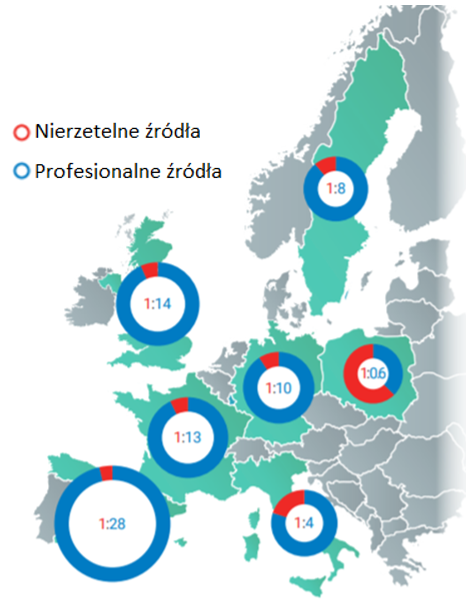
\includegraphics[width=0.5\linewidth]{img/EUMapJunkNews.PNG}
	\caption{Porównanie liczby treści ze źródeł nierzetelnych oraz profesjonalnych w wybranych państwach UE. źródło: \cite{marchal2019junk}}
	\label{fig:EUMapJunkNews}
\end{figure}
\par
Dodatkowo rozsiewanie fałszywych informacji może mieć tak tragiczne skutki jak afera Pizzagate\,\footnote{\url{https://www.nytimes.com/2016/12/05/business/media/comet-ping-pong-pizza-shooting-fake-news-consequences.html}}. Pewien człowiek uwierzywszy w\,teorię spiskową na temat mafii pedofilskiej powiązanej z\,Hillary Clinton wszedł uzbrojony do pizzerii, w\,której miał się odbywać nielegalny proceder i \,otworzył ogień. Na szczęście w\,zajściu nikt nie ucierpiał. Mimo, że przytoczony przykład jest skrajną sytuacją, pokazuje jak łatwo jest manipulować jednostkami. Największy problem pojawia się, jeśli uda się zmanipulować całą masą ludzi. 
\subsection{Podsumowanie problemu}
Fałszywe informacje są często bardzo trudne do wykrycia a\,wciąż rozwijające się algorytmy mogą być używane do szerzenia ich na ogromną skalę. Coraz częściej zaczynamy mówić o problemie wiarygodności w\,dostarczanych nam mediach. Użytkownicy korzystający z\,platform społecznościowych do czytania wiadomości też już zauważyli ten problem. Według najnowszych badań Pew 57\% użytkowników uważa takie informacje za niedokładne \cite{PewNewsUse2018}. Za główne problemy takiego zjawiska wskazują stronniczość polityczną oraz niską jakość publikowanych treści. Nie bez znaczenia jest też zachowanie innych użytkowników. 
\par Żmudne zadanie neutralizacji fałszywych informacji prowadzą już od dawna dedykowane temu portale amerykańskie. W\,polskim Internecie powstał serwis Demagog, który za cel stawia sobie sprawdzanie prawdziwości wypowiedzi polityków. Do walki z\,rozszerzającymi się fałszywymi informacjami włącza się również technologia. Powstaje coraz więcej prób zautomatyzowania wykrywania niewiarygodnych źródeł i\,artykułów mówiących nieprawdę. Automatyczne wykrywanie fake news jest to przewidywanie szans, że konkretny artykuł jest intencjonalnie fałszywy \cite{threeTypeOfFakes2015}. Niestety w\,tak szybko rozwijającym się środowisku jest to zadanie co najmniej trudne. Nie istnieją jeszcze wystarczająco dobre rozwiązania. Należy więc szukać nowych i\,dodatkowo rozszerzać je na inne języki oprócz języka angielskiego. 
       
\newpage % Rozdziały zaczynamy od nowej strony.
\section{Przegląd istniejących rozwiązań klasyfikacji informacji}
W poniższym rozdziale przedstawione zostaną wybrane metody służące do klasyfikacji informacji pod względem zawierania w\,nich prawdy lub fałszu. Istnieją dwa główne typy mechanizmów: manualny - wymagający pracy człowieka oraz automatyczny gdzie do klasyfikacji używane są różne typy algorytmów lub technik uczenia maszynowego. Automatyczne dodatkowo można wyraźnie rozróżnić pod kątem danych jakie są używane w\,celu klasyfikowania treści. 
\subsection{Rozwiązania manualne} \label{rozwiazania-manualne}
Do tej grupy zostały zakwalifikowane rozwiązania które w\,dużej mierze lub całkowicie polegają na pracy człowieka. Praca ta polega na manualnej decyzji osoby czy przedstawiony jej tekst zawiera prawdę czy jest dezinformujący. Sposoby tej pracy różnią się zaangażowaniem oceniającej osoby. Jako eksperta traktujemy osobę która poświęca czas i\,posiadaną wiedzę aby poprzeć swoją opinię dowodami z\,wiarygodnych źródeł. Innym sposobem jest użycie tzw. crowdsourcingu który polega na zbieraniu opinii dużej liczby użytkowników, którzy niekoniecznie są całkowicie wiarygodni. 
\subsubsection{Praca ekspertów}
Badanie rzetelności faktów zawartych w\,artykułach lub w\,wypowiedziach osób publicznych jest często zadaniem skomplikowanym oraz czasochłonnym. Są jednak inicjatywy poświęcone wykrywaniu fałszu lub niepełnej prawdziwości w\,publikowanych informacjach. Jednymi z\,najbardziej popularnych stron zajmujących się taką weryfikacją są Politifact\footnote{\url{https://www.politifact.com}} oraz Snopes\footnote{\url{https://www.snopes.com}} . Podejmują one głównie tematy związane ze polityką Stanów Zjednoczonych. Ich działanie polega na zatrudnianiu niezależnych dziennikarzy, których zadaniem jest wyszukiwanie źródeł weryfikujących wiarygodność informacji podawanych w\,sieci. Oceniają oni daną informację według ustalonej klasyfikacji. Aby być samemu być wiarygodnym zawsze podają źródła zarówno sprawdzanej informacji jak i\,materiałów użytych do wydania oceny. Dzięki temu użytkownik sam może zweryfikować swoją opinię. 
\par To rozwiązanie mimo oczywistych plusów, jakimi jest rzetelność i\,przejrzystość weryfikacji wierzytelności ma też znaczące minusy. Wymaga ono dużych nakładów pracy wykonanej przez specjalnie zatrudnionych w\,tym celu ekspertów. Metoda ta jest również czasochłonna zwłaszcza przy niejasnych przypadkach. Zwiększa to ryzyko, że kłamliwa informacja zostanie rozpowszechniona wśród większej liczby osób zanim zostanie zweryfikowana. Ponadto działanie takiego rozwiązania opiera się na założeniu, że użytkownicy czytają jedną z\,weryfikujących stron, co wymaga większego zaangażowania i\,może powodować pewną niedogodność dla standardowego odbiorcy. 
\subsubsection{Crowdsourcing}
Inną stosowaną metodą na wykrywanie fałszu jest crowdsourcing. Istnieją rozwiązania, które zbierają opinie użytkowników na temat prawdziwości lub nieszczerości konkretnych wypowiedzi umieszczanych w\,Internecie. Dzięki temu mogą one ostrzegać innych użytkowników przed zbytnią ufnością do czytanego źródła. Takie podejście wykorzystuje na przykład projekt fakenewsdetector.org\footnote{\url{https://fakenewsdetector.org/en}}. Jest to projekt opensource, który stworzył wtyczkę internetową o tej samej nazwie. Połączył on opisaną wyżej metodę jako zbieranie danych do uczenia maszynowego. Dzięki temu uczy się klasyfikować informacje świeżo opublikowane, które nie zdążyły być jeszcze przeczytane przez żadnego użytkownika. 
\par Fiskkit\footnote{\url{https://fiskkit.com}} jest platformą, która daje większe możliwości dyskusji nad artykułem niż przeciętne medium z\,artykułami. Platforma nie zawiera własnych artykułów, ale pozwala użytkownikom na importowanie ich z\,dowolnego źródła i\,daje możliwość dyskusji bezpośrednio nad każdym osobnym zdaniem w\,danym tekście. Użytkownicy mogą więc wskazywać dokładne fragmenty które uważają za fałszywe lub zbyt uproszczone.
\par Dużym minusem wykorzystania corwdsourcingu w\,ocenianiu prawdziwości artykułów powinien być brak zaufania do mas użytkowników. Osoby udzielające swojej opinii mogą być skrajnie stronnicze tak samo jak są przy udostępnianiu niepewnych informacji na portalach społecznościowych.

\subsection{Rozwiązania automatyczne}
Poniżej przedstawię kilka wybranych rozwiązań informatycznych działających w\,kieru- nku wykrywania fałszu lub stronniczości w\,artykułach i\,mediach społecznościowych. 
Warto na początku zaznaczyć, że większość istniejących prac skupia się na treściach intencjonalnie fałszywych, odrzucając teorie spiskowe, plotki, ponieważ te z\,definicji są trudniejsze do określenia czy są całkowicie fałszywe czy zawierają prawdę. Z\,rozpoznawania powinno się też wyłączyć satyrę, ponieważ ta działa na innych prawach. Portale publikujące teksty satyryczne zazwyczaj bezpośrednio podają do wiadomości użytkownika, że zawierają treści humorystyczne i\,informacje w\,nich zawarte nie powinny być traktowane poważnie.

\subsubsection{Style-based}
Rozważania nad używaniem metod przetwarzania języka naturalnego wywodzi się z\,założenia, że artykuły, które szerzą intencjonalną dezinformację różnią się stylem od artykułów prawdziwych. Może się to ujawniać na przykład w\,bardziej emocjonalnym słownictwie, poruszanych tematach lub skrajnej stronniczości.
\par Częstym zabiegiem wykorzystywanym do szerzenia dezinformacji w\,artykułach jest wykorzystywanie chwytliwego tytułu. Taka metoda często ma za zadanie zwabić czytelnika na kliknięcie w\,artykuł (tzw. clickbait). Oprócz takiego zastosowania równie często zdarza się, że sam tytuł może wyrażać fałszywe stwierdzenie natomiast treść artykułu naprostowuje je w\,stronę prawdy, użytkownik jednak nie dowie się o omylności tytułu, jeśli nie zdecyduje się przeczytać całości. W\,2017 zorganizowany został konkurs FakeNewsChallange\footnote{\url{http://www.fakenewschallenge.org}}, którego pierwszym etapem było stworzenie rozwiązania wykrywającego w\,jaki sposób treść artykułu odnosi się do jego tytułu. Może on bowiem zgadzać się lub nie zgadzać z\,tytułem. Artykuł może też omawiać dany temat ale nie wyrażać własnej opinii, możliwe jest też że treść dotyczy innego tematu niż tytuł. Rozwiązanie, które zostało ocenione najlepiej zostało stworzone przez grupę o nazwie Solat in the Swen. Stworzyli oni model oparty na połączeniu drzew decyzyjnych oraz głębokich sieci neuronowych. 
\par
Także w\,Polsce powstało badanie mające na celu sprawdzenia możliwości wykorzystania wiedzy psycholingwistycznej w\,celu rozpoznawania zdań zawierających fałsz\cite{wawer2019fact}. W\,tym celu zebrano 400 stwierdzeń od 200 uczestników. Jednak aby wykonać to badanie zdania zebrane w\,języku polskim zostały przetłumaczone na język angielski używając Google Translate. Mimo to dla zdań o silnie spolaryzowanych tematach otrzymano lepsze wyniki niż w\,przypadku testowania poprzez factchecking z\,wykorzystaniem portalu Wikipedia. 

\subsubsection{Knowladge-based}
Aby automatycznie wykrywać, czy informacja jest prawdziwa czy też nie można zastosować dostępne ustrukturalizowane bazy wiedzy takie jak DBpedia , która pobiera dane z\,Wikipedii tworząc sieć semantyczną. Jej celem jest uporządkowanie wiedzy, jaka istnieje w\,Internecie w\,formie grafu wiedzy.  Takie podejście sprawdziło się przy sprawdzaniu krótkich twierdzeń na temat historii, geografii czy rozrywki\cite{ciampaglia2015computational}. Wykorzystano tam zależność między bliskością zagadnień w\,grafie wskazujących na prawdziwość zdania, w\,którym występują.
\par 
Wizualizację takiej metody przedstawiono na rysunku \ref{fig:barackObama} gdzie bazując na informacjach z\,Wikipedii starano się ustalić czy zdanie "Barack Obama jest muzułmaninem" jest prawdziwe czy fałszywe. Po lewej znajduje się informacja o postaci pobrana bezpośrednio z\,Wikipedii a\,po prawej ścieżka jaką przeszedł algorytm aby połączyć ze sobą dwa pojęcia: Barack Obama oraz islam. Liczby w\,nawiasach oznaczają ilość połączeń jaki posiada dana strona. Im wyższa to liczba tym niższą daje wartość do obliczenia końcowej wartości prawdopodobieństwa prawdy w\,badanym zdaniu. 

\begin{figure}[!h]
	\centering 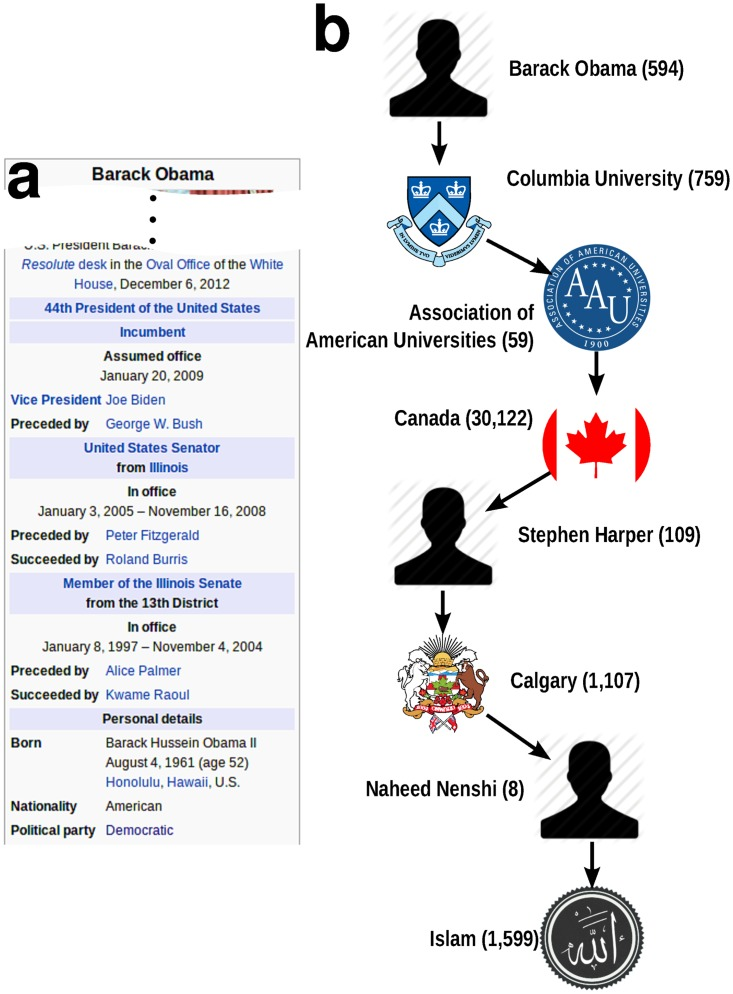
\includegraphics[width=0.5\linewidth]{img/barackObamaIsAMuslimNew.jpg}
	\caption{Wizualizacja zastosowania artykułów w\,Wikipedii do określenia prawdziwości stwierdzenia. Źródło: \cite{ciampaglia2015computational}}
	\label{fig:barackObama}
\end{figure}
\par

\subsubsection{Context-based}
To podejście skupia się nie na treści prezentowanej informacji ale na jej kontekście. Jako kontekst można traktować autora tej informacji, serwis na którym się znajduje lub komentarze pozostawione przez odbiorców. Świetnym źródłem do zbierania tego typu informacji o kontekście są media społecznościowe. Ich idea polega na tym aby użytkownicy ingerowali w\,publikowane treści poprzez komentowanie, prowadzenie dyskusji i\,udostępnianie informacji większej grupie odbiorców.
\par
W obecnych czasach bardzo duże znaczenie mają media społecznościowe. Według badań z\,2018 roku 68\% ankietowanych pobiera wiedzę o aktualnych wydarzeniach właśnie z\,takich źródeł \cite{PewNewsUse2018}. Jest to wygodne i\,szybkie jednak bardzo podatne na manipulacje. Można jednak wykorzystać sieci zależności jakie tworzą źródła publikujące informacje z\,ich odbiorcami. Praca pod tytułem Some like it Hoax\cite{tacchini2017some} skupiła się na działalności użytkowników platformy Facebook jakim są ’polubienia’ postów. Projekt pobrał 15,500 postów polubionych przez ponad 900 tysięcy użytkowników. Aby wykrywać potencjalny fake news wykorzystał stworzony wcześniej podział stron na naukowe oraz o tematyce konspiracyjnej\cite{bessi2015science}. Wykorzystując fakt, że większość użytkowników ograniczała swoją aktywność tyko do postów należących do tylko jednej z\,tych kategorii, ale istnieje też niemała grupa akceptująca oba rodzaje stron możliwe było osiągnięcie bardzo wysokich wyników klasyfikacji postów do odpowiedniej kategorii. 
\par
Powstał również portal o nazwie Hoaxy\cite{shao2016hoaxy} na którym można prześledzić w\,formie grafu jak udostępniane są posty publikowane na Twitter. Dzięki tej aplikacji można zobaczyć, jak rozprzestrzenia się wskazany przez nas post, w\,czasie między kolejnymi użytkownikami serwisu. Przykład wykorzystania tej aplikacji ukazano na rysunku \ref{fig:hoaxyTrump}. Znajduje się na nim wizualizacja sieci rozprzestrzeniania się wiadomości opublikowanej pierwotnie na koncie Donalda Trumpa dnia 03.05.2019. W\,czasie dwóch dni informacja ta została przekazana ponad 22 tysiące razy.
\begin{figure}[!h]
	
	\centering 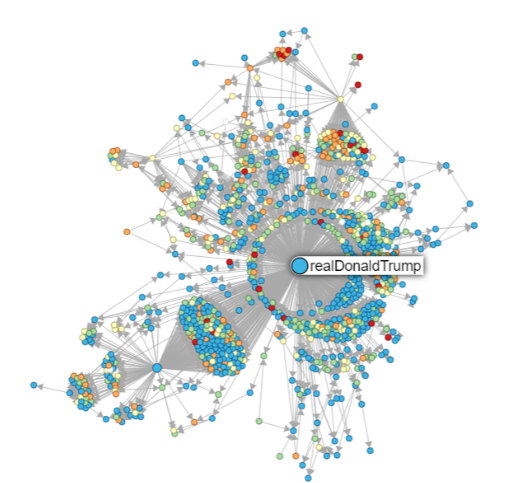
\includegraphics[width=0.7\linewidth]{img/hoaxy.png}
	\caption{Sieć rozprzestrzeniania się wiadomości na platformie Twitter na przykładzie wiadomości Donalda Trumpa. Źródło: \url{https://hoaxy.iuni.iu.edu}}
	\label{fig:hoaxyTrump}
\end{figure}
\par
Innym podejściem do klasyfikacji źródeł publikujących informacje jest wykorzystanie odniesień jakie robią między sobą strony internetowe. Taką metodę wykorzystywał Pagerank działający dla Google. Wyznaczając rangę ważności strony brał on pod uwagę rangę stron, do których dana storna się odwoływała. Innym algorytmem wykorzystującą sieć skierowaną którą tworzą odniesienia jakie występują między stronami jest HITS. Opisuje on dwa typy stron: autorytety i\,koncentratory. Autorytetem jest strona, która jest często cytowana przez inne strony, natomiast koncentratorem jest strona, która wskazuje na wiele ważnych stron. Fakt, że strony internetowe zawierają odniesienia do innych stron można wykorzystać też do badania wiarygodności portali internetowych pod względem prawdziwości publikowanych informacji. Badania wykazały, że wykrywanie kłamliwych źródeł w\,takim grafie odbywa się z\,dużo większym sukcesem niż próba wykrycia tego przy zastosowaniu metod lingwistycznych bezpośrednio na publikowanych artykułach\cite{fairbanks2018credibility}. Wykorzystano w\,nich bazę danych pochodzącą z\,The Global Database o Events Language and Tone\footnote{\url{https://www.gdeltproject.org}}. Z\,pobranych artykułów podających linki zewnętrzne stworzono graf zawierający ponad 19 tysięcy unikalnych źródeł połączonych ponad 32 tysiącami linków. Oznaczenia wiarygodności dokonano na poziomie źródła, wykorzystano do tego istniejące oceny stron wykonane przez portal Media Bias Fact Check\footnote{\url{https://mediabiasfactcheck.com}}. Dzięki wykorzystaniu odpowiedniego algorytmu propagacji nie było wymagane, aby wszystkie źródła w\,grafie miały na wstępie zadeklarowaną ocenę. 
\subsection{Przegląd istniejących baz danych}
Poniżej zostaną przedstawione wymagania, które musi spełniać zbiór danych aby było możliwe użycie go w\,celu badań możliwości automatycznej klasyfikacji informacji. Dodatkowo zostaną zaprezentowane przykładowe bazy danych, które są udostępnione w\,tym celu oraz posiadają już sprawdzone etykiety.
\subsubsection{Wymagania korpusu danych}
Przy rozpoczynaniu pracy nad automatycznym wykrywaniem fałszywych informacji najpierw należy posiadać odpowiedni zbiór odpowiednio oznaczonych danych. Takimi danymi mogą być całe artykuły, tytuły takich artykułów czy posty w\,mediach społecznościowych. Ważne jest jednak, aby taki korpus był spójny i\,trzymał się również kilku innych zasad. Zestaw dziewięciu takich zasad zebrali w\,swojej pracy Rubin, Conroy i\,Chen\cite{rubin2015deception}.
\begin{enumerate}
    \item Korpus zawsze powinien składać się z\,zarówno prawdziwych jak I fałszywych instancji. Jest to niezbędne, aby można było podać go jako zbiór służący do nauki modelu.
    \item Jeśli chcemy zastosować NLP dane powinny występować w\,formie tekstu.
    \item Powinniśmy mieć pewność na temat poprawnego oznakowania naszych informacji jako prawdziwe lub fałszywe. O ile jest to prostsze w\,przypadku brania danych ze źródeł uważanych powszechnie za wiarygodne, tak w\,przypadku korzystania z\,metody crowdsoursingu należy oznaczać jedynie prawdopodobieństwo prawdziwości informacji.
    \item Należy zwrócić uwagę, aby teksty były podobnej długości. Nie można mieszać krótkich form takich jak posty w\,mediach społecznościach z\,długimi artykułami.
    \item Teksty powinny być homogeniczne w\,stylu oraz tematyce. Należy zbierać te same typy publikowanych informacji w\,rozdzieleniu na typ pisarski, różnicą jest czy autorem jest dziennikarz lub czy jest pisane stylem potocznym. Ważne jest wybranie z\,góry określonej tematyki lub zbioru tematów, o których będą mówić nasze zebrane informacje.
    \item Należy określić dokładny zakres czasowy z\,którego będą zebrane informacje.
    \item Powinno się zwrócić również uwagę czy cel opublikowania tych informacji był ten sam. Nie powinno się na przykład mieszać standardowych tekstów z\,tymi o zabarwieniu humorystycznym lub satyrycznym.
    \item Ważne są pragmatyczne cechy źródeł tekstów takie jak publiczny i\,bezpłatny dostęp do nich oraz łatwość w\,przetwarzaniu.
    \item Warto zwrócić uwagę na różnice językowe i\,kulturowe.

\end{enumerate}


\subsubsection{Przykładowe bazy danych}
    \par LIAR
    - dane pobrane przez API udostępnione przez PolitiFact. Są to krótkie zdania pochodzące z\,różnego rodzaju źródeł takich jak artykuły, wywiady lub przemowy polityków. Każde zdanie z\,bazy ponad 12 tysięcy zostało ocenione manualnie przez człowieka\cite{wang2017liar}.
    \par CREDBANK  - baza zawierająca 60 milionów postów z\,platformy Twitter obejmująca zakres trzech miesięcy w\,2015 roku \cite{mitra2015credbank}. Posty te zostały zakwalifikowane do odpowiedniego z\,ponad tysiąca wydarzeń a\,każde wydarzenie zostało oznaczone przez 30 użytkowników Amazon Mechanical Turk .
    \par BuzzFeedNews
    \footnote{\url{https://github.com/BuzzFeedNews/2016-10-facebook-fact-check/tree/master/data}} 
    - zawiera posty z\,Facebooka z\,tygodni w\,roku 2016 bliskich wyborom prezydenckim w\,USA. Każdy post był oceniony przez dziennikarzy BuzzFeed. Posty były pobrane z\,niewielkiej ilośći zróżnicowanych źródeł.
    \par BD Detector
    \footnote{\url{https://www.kaggle.com/mrisdal/fake-news}}
    - dane pobrane przez wtyczkę wyszukiwarki o tej samej nazwie. Szuka ona linków na stronach i\,sprawdza powiązania z\,manualnie stworzoną bazą danych na temat niewiarygodnych źródeł.  Aplikacja nie jest już jednak utrzymywana przez deweloperów.
    \par The Global Datbase of Events Language and Tone
    \footnote{\url{https://www.gdeltproject.org}}
    – projekt, który pobiera informacje pojawiające się na platformach z\,ponad 100 krajów świata. Jego celem jest monitorowanie wydarzeń na świecie i\,identyfikuje związane z\,tymi wydarzeniami osoby, miejsca i\,informacje oraz emocje jakie wywołują one w\,mediach. 
    \par Media Bias Fact Check
    \footnote{\url{https://mediabiasfactcheck.com}}
    - portal dokonujący oceny stronniczości politycznej innych źródeł informacji. Dokonuje również podziału na media naukowe oraz pseudonaukowe. Wskazuje też na źródła skrajnie stronnicze lub wręcz intencjonalnie kłamliwe jak również podaje listę portali określających samych siebie jako satyryczne lub humorystyczne. 



\newpage
\section{Badanie wiarygodności informacji}
W tym rozdziale zostaną przedstawione i opisane badania wiarygodności informacji skupiające się na informacjach związanych z Polską i Unią Europejską. Jako wiarygodność informacji rozumie się prawdopodobieństwo, że dana informacja jest prawdziwa. Wiarygodność źródła oznacz prawdopodobieństwo, że informacje które ono udostępnia są prawdziwe. Jako synonim do małego prawdopodobieństwa prawdziwości będą używane słowa nierzetelny, mało wiarygodny, nieprawdziwy lub dezinformujący. 
\subsection{Rodzaje źródeł informacji}
Centrum badania opinii społecznej CBOS przeprowadziło w\,kwietniu 2019 roku badania dotyczące wiarygodności mediów w\,Polsce. Zostały one przeprowadzone metodą wywiadów bezpośrednich na reprezentatywnej próbie losowej dorosłych liczącej 1064 osoby. CBOS przeprowadziło takie badania już po raz drugi, dzięki czemu można porównać jakie zmiany w\,opinii publicznej nastąpiły w\,ciągu dwóch ostatnich lat\cite{CBOSWiarygodnoscMediow2019}.
\par 
Jednym z\,punktów zainteresowań badania była informacja co jest głównym źródłem czerpania informacji o wydarzeniach w\,kraju i\,na świecie Polaków.  Z\,uzyskanych odpowiedzi wynika, że wzrosło znaczenie Internetu używanego w\,takim celu z\,21\% w\,2017 roku do 27\% w\,2019 roku. Jednocześnie zmalała o sześć procent liczba osób deklarująca telewizję jako główne źródło informacji. Inne źródła takie jak radio i\,prasa są najważniejszym źródłem informacji dla relatywnie niewielkiej grupy. Dodatkowo patrząc na zróżnicowanie społeczne odbiorców poszczególnych mediów można zauważyć, że bardzo duże znaczenie ma wiek. W\,grupie młodych dorosłych (osoby w\,wieku 18-24 lata) 60\% deklaruje, że ich głównym źródłem pobierania informacji jest Internet. Patrząc na takie statystyki śmiało można założyć, że znaczenie Internetu w\,dostarczaniu informacji będzie nadal rosło.


\subsubsection{Zaufanie do informacji w\,mediach}
Na zlecenie Komisji Europejskiej międzynarodowy projekt badania opinii publicznej Eurobarometer w\,2018 roku przeprowadził badania na temat fałszywych informacji w\,Internecie\cite{Eurobarometer4642018}. W\,badaniu pytano obywateli wszystkich krajów Unii Europejskiej w\,tym również Polski jakim stopniu ufają różnym typom mediów. Jako zaufanie uznaje się odpowiedź „całkowicie ufam” oraz „raczej ufam” po-daną przez respondenta na pytanie. Polacy mają największe zaufanie do radia 63\% a\,następnie do drukowanej prasy oraz telewizji (odpowiednio 55\% i\,54\%). Patrząc na media publikujące w\,Internecie największym zaufaniem cieszą się portale informacyjne 45\% a\,najmniej respondentów, bo 34\% ma zaufanie do informacji pobieranych poprzez media społecznościowe oraz aplikacje służące do komunikacji. 
\par
Jednak jak wynika z\,poprzednich badań przeprowadzonych przez Eurobarometr prawie jedna piąta użytkowników Internetu w\,Polsce (19\%) pobiera informacje o wiadomościach korzystając z\,mediów społecznościowych. Warto przy tym zwrócić uwagę, że tylko połowa osób kliknie w\,link, aby przeczytać całość artykułu na jego oryginalnej stronie internetowej\cite{Eurobarometer2016}. Takie zachowanie użytkowników umożliwia nierzetelnym stronom na manipulacje informacjami. Zdarza się bowiem, że tytuł przedstawia informację w\,fałszywy sposób a\,dopiero treść artykułu wyjaśnia jak sytuacja naprawdę wygląda. 
\subsection{Fałszywe informacje w\,Internecie}
Badania skupiające się na opinii Polskich internautów o dezinformacji w\,sieci przeprowadził państwowy instytut badawczy NASK na przełomie marca i\,kwietnia 2019\cite{NASKBezpieczneWybory2019}. Zapytano grupy 1000 internautów czy w\,przeciągu 6 ostatnich miesięcy spotkali się w\,Internecie z\,informacjami, które według ich opinii mogły być sfałszowane lub zmanipulowane. Z\,tych badań wynika, że ponad połowa ankietowanych (56\%) spotkała się z\,takim zjawiskiem w\,Internecie w\,przeciągu ostatniego pół roku od chwili zadanego pytania, w\,tym prawie co czwarta osoba zauważa jakąś manipulację informacją codziennie lub kilka razy w\,tygodniu. Tylko 11\% ankietowanych twierdzi, że nie spotkało się z\,zmanipulowanymi informacjami. Pozostałe osoby nie potrafiły odpowiedzieć na to pytanie w\,twierdzący lub zaprzeczający sposób. Część wyników przedstawiono za pomocą diagramu kołowego na rysunku \ref{fig:NASKwyniki}.
\begin{figure}[!h]
	
	\centering 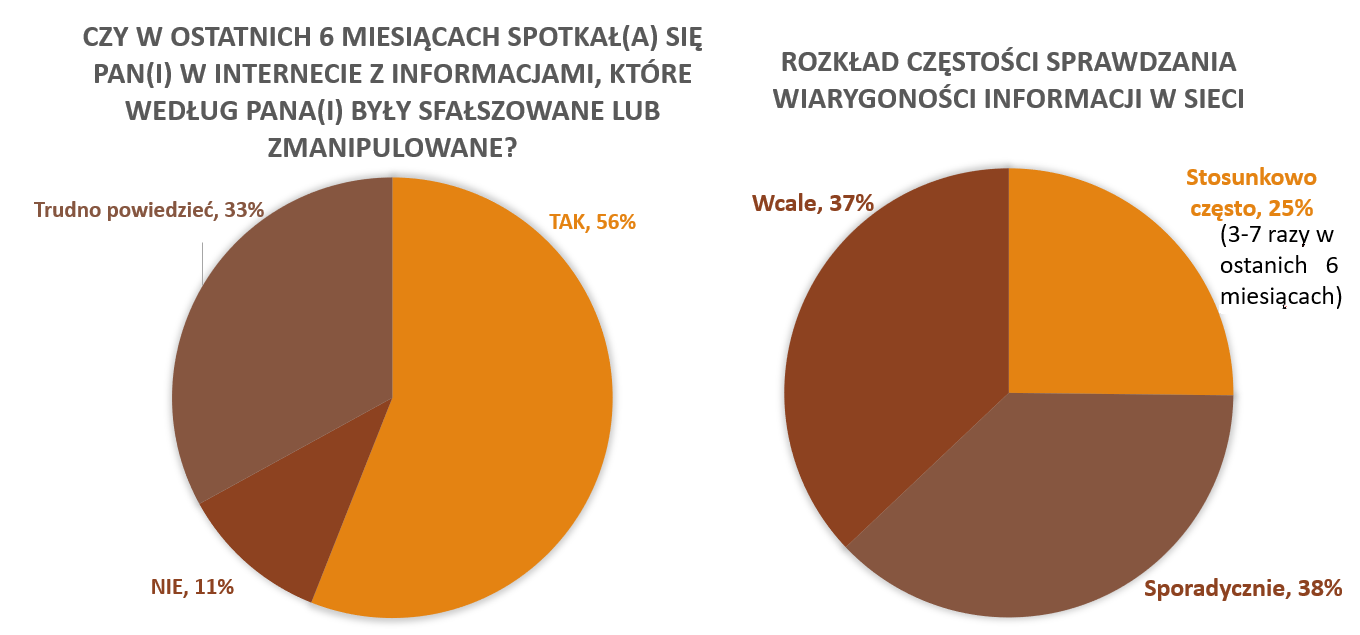
\includegraphics[width=0.9\linewidth]{img/NASKwyniki.PNG}
	\caption{Wybrane wyniki z\,badania opinii Polaków na temat dezinformacji w\,internecie. Opracowanie własne na podstawie źródła: \cite{NASKBezpieczneWybory2019}}
	\label{fig:NASKwyniki}
\end{figure}
\par
\par
Najwięcej respondentów (30\%) jako najczęściej spotykaną przez nich formę dezinformacji i\,manipulacji w\,Internecie określiło fake news, czyli szeroko pojęte fałszywe informacje.  Następnie wskazywano zmanipulowane zdjęcia oraz tzw. trolling czyli celowe prowokowanie do kłótni na forach internetowych poprzez publikowanie nieprawdziwych albo emocjonalnych treści. Jedna piąta ankietowanych nie była jednak w\,stanie powiedzieć jaki typ dezinformacji lub manipulacji najczęściej spotykają.
\par
Tak częste występowanie fałszywych informacji w\,sieci wiąże się z\,tym, że część użytkowników Internetu intencjonalnie lub nieintencjonalnie wchodzi z\,nimi w\,aktywną interakcję przesyłając dalej takie treści lub wyrażając aprobatę poprzez klikanie ‘lubię to’ przy takich publikacjach. Do takiego zachowania w\,czasie ostatniego pół roku przyznało się łącznie prawie 20\% ankietowanych w\,tym 12\% deklaruje, że zrobiło to nie mając świadomości o fałszywości zawartych tam informacji\cite{NASKBezpieczneWybory2019}. 



\subsection{Weryfikacja informacji} \label{badanie-wiarygodnosci-w-internecie}
Rozprzestrzenianie  fałszywych informacji w\,Internecie potęguje fakt, że większość osób nigdy lub tylko sporadycznie weryfikuje czy informacje, które czytają są wiarygodne. Tylko 25\% badanych zadeklarowało, że kilkakrotnie w\,przeciągu ostatniego pół roku sprawdziło wiarygodność czytanej informacji w\,sieci pod kątem treści, źródła lub wiarygodności informacji zawartych na profilu w\,mediach społecznościowych\cite{NASKBezpieczneWybory2019}. Osoby, które najczęściej weryfikują czytane treści internetowe to takie, które często napotykają zmanipulowane wiadomości o tematyce ideologiczno-kulturowej.
\par
Sposoby jakie respondenci najczęściej używają w\,celu oceny wiarygodności informacji znalezionych w\,Internecie można podzielić na 3 grupy metod. Są nimi:
\begin{itemize}
    \item Rzetelność dziennikarska – odbiorcy patrzą na to czy do publikowanej treści podawane są źródła, na których ona się opiera oraz czy zawiera różne punkty widzenia. 
    \item Osobiste zaufanie – bardziej ufamy informacjom, które pochodzą ze źródła, do którego mamy już zbudowane zaufanie lub autorem jest osoba której ufamy. Do tego dołącza również przeświadczenie, że jeśli daną informacje publikuje albo poleca osoba, którą znamy będziemy bardziej skłonny zaufać i\,uwierzyć w\,czytane treści.
    \item Społeczny dowód słuszności – polega ona na tym, że dużą wiarygodność otrzymują informacje, które pochodzą z\,dużego i\,popularnego medium albo gdy dana informacja przekazywana jest przez wiele osób lub mediów jednocześnie.   
\end{itemize}



\subsection{Klasyfikacja wiarygodności źródeł}
Aby powstał jakikolwiek automatyczny sposób wykrywania fałszywych informacji w\,Internecie na podstawie jego kontekstu należy najpierw przygotować odpowiednią klasyfikację. Ocenianie każdego opublikowanego artykułu lub postu z\,wybranego zbioru jest zadaniem niezwykle żmudnym. Należy więc utworzyć mechanizm grupowania ocenianych treści. W\,jednym ze sposobów można uznać, że jeśli konkretne źródło tworzące lub udostępniające treści uznamy za niewiarygodne, można założyć, że wszystkie treści publikowane przez to źródło są niewiarygodne. Takie postępowanie przyjęli twórcy artykułu „Some like it Hoax”\cite{tacchini2017some}, badający zachowania użytkowników portalu Facebook względem postów wystawianych przez strony naukowe oraz o tematyce konspiracyjnej. Podobne podziały dla mediów amerykańskich można znaleźć na wyspecjalizowanych stronach takich jak politifact.com\footnote{\url{https://www.politifact.com/punditfact/article/2017/apr/20/politifacts-guide-fake-news-websites-and-what-they/}},  mediabiasfactcheck.com\footnote{\url{https://mediabiasfactcheck.com}}  lub innych zbiorach stworzonych specjalnie do tego celu. Są to strony wyspecjalizowane w\,sprawdzaniu prawdziwości treści i\,wykrywaniu dezinformacji. 
\par
Większość działań podjętych w\,celu wykrycia nierzetelnych stron internetowych publikujących nieprawdziwe informacje skupia się na treściach powiązanymi ze Stanami Zjednoczonymi Ameryki. Niewiele podobnych inicjatyw istnieje w\,Europie. Nie dziwi to jednak ponieważ, ocenianie całych portali internetowych pod względem ich wiarygodności jest niezwykle wrażliwym tematem i\,jest obciążone olbrzymią odpowiedzialnością. 
\subsubsection{Nierzetelne źródła medialne w\,Europie} \label{nierzetelne-zrodla-eu}
Na skalę europejską takiego działania podjął się zespół Instytutu Informatyki w\,Oxfo- rdzie jako część projektu o nazwie Computational Propaganda project COMPROP. Zespół zajmuje się między innymi analizą w\,jaki sposób automatyzacja działań w mediach społecznościowych wpływa na rozprzestrzenianie treści związanych z\,polityką, mową nienawiści i\,dezinformacji oraz jak to może wpłynąć na manipulowanie opinią publiczną. 
\par
Jeden z\,projektów tego zespołu „Junk news aggregator” powstał z\,intencją pomocy naukowcom i\,dziennikarzom w\,kolejnych badaniach nad problemem dezinformacji w\,Inter- necie. Projekt ten zbierał posty publikowane na platformie Facebook przez strony uznane przez zespół jako publikujące śmieciowe informacje.  W\,swojej pierwszej pracy na temat tego projektu\cite{liotsiou2019junk} wyodrębniono strony uznane przez nich jako śmieciowe których publikowane treści dotyczyły wyborów w\,Stanach Zjednoczonych przeprowadzonych listopadzie 2018. Następnie, aby dać możliwość obserwowania zmanipulowanych informacji dotyczących wyborów do Parlamentu Europejskiego w\,maju 2019 dołączono również kilkadziesiąt portali z\,kilku krajów Europy w\,tym również z\,Polski. Dzięki temu, dostępna jest lista 13-tu\,polskich portali informacyjnych które zespół COMPROP uznał za nierzetelne. 
\subsubsection{Metoda oceny źródeł} \label{metoda-oceny-zrodel}
Przypisywanie kategorii stronom internetowym wykonane było przez ekspertów przygotowanych dla każdego kraju i\,było oparte na stworzonej wcześniej typologii\cite{neudertpolarization2018}. W\,przy- padku nierzetelnych źródeł medialnych jest pięć kryteriów, jeśli źródło spełnia przynajmniej trzy z\,nich było zakwalifikowywane jako należące do kategorii ‘śmieciowe’. Poniżej przedstawiam opis tych pięciu kategorii oraz dodatkowej szóstej będącej zależnej od poprzednich:
\begin{itemize}
    \item Profesjonalizm – są to źródła, które nie spełniają standardów profesjonalnego dziennikarstwa. Często nie podają informacji na temat autorów, redaktorów czy wydawców. Brakuje im przejrzystości i\,odpowiedzialności za publikowane treści. Nie publikują korekt do obalonych informacji.
    \item Styl – portale które używają emocjonalnego języka, hiperbol lub mylących tytułów. Wstawiają dużo niepowiązanych zdjęć, często wzbudzających emocje w\,odbiorcach.
    \item Wiarygodność – publikujące fałszywe informacje lub teorie spiskowe. Nie sprawdzają innych źródeł ani prawdziwości udostępnianych przez siebie informacji.
    \item Stronniczość – publikowane przez nich treści są silnie stronnicze ideologicznie lub politycznie. Raportowane informacje zazwyczaj zawierają opiniotwórczy komentarz.
    \item Imitacja – są to portale które w\,swojej formie przypominają rzetelne źródło informacyjne upodabniając używaną czcionkę i\,styl. Powołują się na źródła uznawane za wiarygodne, ale publikują tylko własną opinię lub bezwartościowe treści.
    \item Agregacja – strony, które udostępniają artykuły stworzone przez źródła, które zostały na podstawie poprzednich kategorii uznane za śmieciowe.
\end{itemize}

\subsection{Informacja i\,dezinformacja w\,mediach społecznościowych}
\label{istniejace-badania-twitter}
Najbardziej popularnym i\,najczęściej używanym portalem społecznościowym w\,Polsce jest Facebook. Jest on drugą najczęściej odwiedzaną domeną zaraz po google.com. Prawie trzy czwarte polskich internautów, czyli 21 milionów Polaków jest jego użytkownikami a\,codziennie średnio ponad 7 milionów Polaków odwiedza ten portal\cite{GemiusInternet2019}. Drugim najbardziej popularnym portalem społecznościowym jest Instagram będący serwisem do publikowania zdjęć a\,na trzecim miejscu plasuje się Twitter z\,liczbą prawie 5 milionów polskich użytkowników\cite{GemiusSerwisy2019}. Mimo, że Twitter jest rzadziej używany przez ogół internautów jest ważną platformą dla polityków, działaczy społecznych oraz dziennikarzy\cite{gorwa2017computational}. Dzięki swojej formie mikroblogów jest wygodnym narzędziem do przekazania publiczności informacji, opinii lub komentarza w\,krótkiej formie jaką jest Tweet.
\subsubsection{Badanie typów informacji na Twitterze}
Przed wyborami do Parlamentu Europejskiego COMPROP przeprowadziło badania na temat typów informacji rozprzestrzenianych na platformach społecznościowych takich jak Twitter i\,Facebook\cite{marchal2019junk}. Pod uwagę wzięto siedem grup językowych w\,tym również polski. Dzięki odpowiednim hashtagom zebrano Tweety związane z\,wyborami a\,następnie wyodrębniono linki URL. Tak uzyskane źródła zakwalifikowano do pięciu typów: Profesjonalne portale informacyjne, profesjonalne źródła rządowe, śmieciowe portale, inne portale informacyjne oraz inne źródła. Dzięki temu można było zbadać które źródła mają największą popularność wśród użytkowników mediów społecznościowych. Okazało się, że w\,zebranym zbiorze Tweetów tylko 4\% zawiera w\,sobie link do źródła oznaczonego jako śmieciowe. Jednak w\,podzbiorze polskojęzycznym było to aż 20\% badanych Tweetów. Należy pamiętać, że nie brano pod uwagę kontekstu z\,jakim opublikowany był każdy Tweet, możliwym jest, że mógł zawierać sprostowanie lub niezgodę z\,zawartą w\,podlinkowanym artykule. Nie mniej oznacza to, że według powyższych badań co piąty polskojęzyczny Tweet zawierał link do nierzetelnego źródła.  
\subsubsection{Rozprzestrzenianie dezinformacji na Twitterze}
Rozprzestrzenianie się nieprawdziwych informacji i\,plotek na platformie Twitter jest poważnym problemem. Porównując popularność publikowanych plotek zauważono, że te które okazują się zawierać nieprawdę mają o 70\% większe prawdopodobieństwo ponownego udostępnienia przez innych użytkowników w\,porównaniu do tych które mówią prawdę\cite{vosoughi2018spread}. Tweety zawierające nieprawdę rozprzestrzeniają się szybciej i\,docierają do większej ilości użytkowników. Zauważono, że użytkownicy częściej udostępniają wiadomości, które są nowe i\,oryginalne, a\,fałszywe plotki często takie właśnie są. 
\par
Podczas innego badania przyjrzano się problemowi botów, czyli kont sterowanych nie przez człowieka, ale przez algorytm\cite{gorwa2017computational}. Przy użyciu metody heurystycznej ze zbioru ponad 10 000 kont wyodrębniono 500 kont przy których istnieje podejrzenie, że nie są autentyczne. Okazuje się, że te 5\% kont opublikowało 33\% zebranych Tweetów o\,tematyce politycznej. Pokazuje to jak duży wpływ na treści publikowane na platformach społecznościowych mogą mieć konta stworzone specjalnie w\,celu rozpowszechniania konkretnych treści. 

\newpage
\section{Projekt badania}
\subsection{Opis}
W ramach tej pracy stworzono projekt mający na celu zbadać skalę problemu jaką są nierzetelne informacje w\,mediach społecznościowych oraz sprawdzenie skuteczności automatycznej klasyfikacji informacji w\,oparciu o dane kontekstowe.  W\,tym celu skupiono się na polskojęzycznych mediach publikujących na platformie Twitter oraz grupie ich odbiorców. Do analizy zostały wybrane media mogące być zaklasyfikowanymi ze względu na ich rzetelność. Ustalenie klas danych testowych oparto na pracy zespołu uniwersytetu Oxford wskazującej nierzetelne media polskojęzyczne. Przeciwstawiono je mediom profesjonalnym oraz o dużej liczbie odbiorców tzw. Mainstream media.
\subsubsection{Cel projektu}
Pierwszym celem tego projektu jest zbadanie jak popularne są treści publikowane przez nierzetelne media w\,porównaniu do tych mainstreamowych. Zostanie to dokonane poprzez badanie częstotliwości zamieszczania nowych treści, wielkość grupy odbiorców i\,przede wszystkim skalę rozprzestrzeniania się tych informacji biorąc pod uwagę bezpośrednie udostępnienia użytkowników. Zostaną również przeanalizowane wzajemne powiązania między badanymi kontami oraz domeny, które są zamieszczane w\,ich postach.
\par
Drugim celem jest sprawdzenie możliwości automatycznej klasyfikacji postowanych informacji na podstawie danych o użytkownikach je udostępniających. Badanie to jest oparte na pracy Some like it hoax, w\,której badając posty na facebooku i\,użytkowników wchodzących z\,nimi w\,interakcje otrzymało bardzo wysokie wyniki klasyfikacji. W\,celu odtworzenia badania na danych polskojęzycznych zostaną użyte te same algorytmy. Badanie ma wykazać czy dla omawianych danych możliwa jest taka klasyfikacja. Dodatkowo, zostanie zbadane jaka liczba danych wystarczy, aby taką klasyfikację przeprowadzić z\,zadowalającą dokładnością. 


\subsection{Wybór platformy social media}
Dwoma największymi mediami społecznościowymi w\,Polsce udostępniającymi funkcję dzielenia się informacjami tekstowymi przez użytkowników są Facebook oraz Twitter\,\cite{GemiusInternet2019}. Platformy te były już wykorzystywane w\,celu zbierania danych do badań, ponieważ są doskonałym źródłami, z\,których można uzyskać wiedzę na temat preferencji użytkowników. Między innymi z\,tych powodów postanowiono przyjrzeć się możliwościom jakie dają wystawione przez nie API, w\,celu uzyskania danych do badań przeprowadzanych w\,tej pracy.

\subsubsection{Facebook API}
Czytając prace badawcze na temat fałszywych informacji z\,ostatnich lat wiele z\,nich wykorzystuje jako źródło do pobrania danych służących analizie tego zagadnienia, platformę Facebook oraz należące do niej API\footnote{\url{https://developers.facebook.com}}. Było ono wygodnym narzędziem pozwalającym na pobranie informacji o publicznym koncie takie jak listy osób, które je ‘lubią’ lub obserwują. Istniała również możliwość pobierania publicznych postów opublikowanych na dowolnym publicznym koncie wraz z\,podłączonymi komentarzami, reakcjami oraz statystykami udostępnień. Użycie tych funkcji było udostępnione dla każdego uwierzytelnionego użytkownika, tak jak dostępne są dla niego w\,przypadku korzystania z\,platformy lub aplikacji mobilnej. Dzięki darmowemu oraz wszechstronnemu dostępowi do informacji publikowanych jako publiczne przez użytkowników Facebook API było wygodnym narzędziem służących do celów zbierania danych o informacjach publikowanych w\,mediach społecznościowych oraz ich popularności wśród odbiorców. Dzięki temu powstało kilka prac podejmujących próbę rozpoznania wielkości problemu jakim są fałszywe informacje w\,mediach społecznościowych oraz szukających rozwiązania na ich automatyczne rozpoznawanie. 
\par
Niestety wraz ze zmianami wprowadzonymi do Facebook API na koniec kwietnia 2019 roku został zamknięty dostęp do części usług\footnote{\url{https://developers.facebook.com/blog/post/2019/04/25/apiupdates/}}. Obecnie pobieranie informacji poprzez API możliwe wyłącznie dla kont których uwierzytelniony użytkownik jest właścicielem lub administratorem.
\subsubsection{Twitter API}
Platforma Twitter również posiada swoje API\footnote{\url{https://developer.twitter.com/en}}. Może ono służyć zarówno do łatwiejszego prowadzenia własnego konta, uprawiania marketingu lub zbierania danych do analizy. Istnieje kilka projektów oraz prac badawczych wykorzystujących dane pobrane przez Twitter API do badania problemu rozprzestrzeniania się nierzetelnych informacji w\,social mediach\,\cite{marchal2019junk}\cite{gorwa2017computational}\cite{vosoughi2018spread}. Twitter działa na metodzie mikroblogów co oznacza, że każdy użytkownik może publikować posty które inni użytkownicy udostępniają. Daje więc ona dostęp do interesujących mnie informacji.
\par
Powyższe api posiada jednak pewne ograniczenia. Pierwszym z\,nich jest konieczność posiadania konta na Twitterze dzięki któremu można utworzyć konto dla deweloperów. Każdy dostęp do API zabezpieczony jest poprzez standard autoryzujący OAuth. Aby uzyskać prywatny klucz należy wypełnić formularz informując jak i\,w jakim celu będziemy używać tego API oraz czy i\,w jaki sposób zamierzamy przechowywać, przetwarzać oraz publikować uzyskane dane.
Kolejne ograniczenie dotyczy dostępu do funkcjonalności. Twitter API posiada trzy poziomy, gdzie tylko standardowy jest darmowy. Kolejne poziomy, premium oraz enterprise, przeznaczone są dla firm gotowych zainwestować w\,bardziej zaawansowane rozwiązania. Poziom standard daje jednak dostęp do wystarczającej liczby funkcjonalności, aby umożliwić przeprowadzaną w tej pracy analizę. 
\par
Trzecim, najbardziej uciążliwym ograniczeniem, są limity liczby możliwych zapytań lub dostarczonych danych. Większość endpointów ma nałożoną maksymalną liczbę wywołań którą można dokonać do nich w\,ciągu 15 minut używając jednego klucza autoryzującego. Innym rodzajem ograniczenia ilościowego zastosowanego na wybranych endpointach jest maksymalna liczba jednostek obiektów które możemy otrzymać w\,odpowiedzi. Przykładem takiego ograniczenia jest zapytanie o posty danego użytkownika, które zwraca maksymalnie 3200 ostatnio opublikowanych postów użytkownika.
\subsubsection{Użyte enpointy i ich ograniczenia}
W tabeli poniżej przedstawiono informacje o funkcjonalnościach Twitter API użytych do pobrania danych oraz informacje o ich ewentualnych ograniczeniach ilościowych.  

\begin{table}[!h] \label{tab:endointytwitter} \centering
\caption{Informacje o użytych enpointach Twitter API.}
\begin{tabular} { | m{4,5cm} | m{3,5cm}| m{4,5cm} | } \hline
Opis & Twitter Enpoint & Ograniczenia \\  \hline \hline
Pobierz informacje o\,użytkowniku & GET users/show & 900 zapytań / 15 minut \\ \hline
Pobierz listę identyfikatorów followersów \mbox{użytkownika} & GET followers/ids & 15 zapytań / 15 minut \\ \hline
Pobierz tweety użytkownika & GET statuses/ user\_timeline & Max 3200 najnowszych tweetów \mbox{100 000 zaptań /dzień} \\ \hline
Pobierz listę identyfikatorów retweeterów tweeta & GET statuses/ retweeters/ids & Max 100 identyfikatorów dla tweeta \mbox{75 zapytań / 15 min} 
 \\ \hline
\end{tabular}
\end{table}



\subsection{Opis implementacji pobrania danych}
Aby dokonać pobrania danych stworzono system informatyczny dedykowany do tego zadania. Użyto w tym celu języka Java z zastosowaniem framework Spring Boot. Podjęto taka decyzje ponieważ jest to język dostosowany do zadania jakim jest wysyłanie zapytań do zewnętrznego api oraz zapisywanie danych do baz danych oraz jest dobrze znany autorowi.  
\par
Dla ułatwienia pracy przy korzystaniu z\,Twitter API\footnote{\url{http://twitter4j.org}} użyto ogólnodostępną bibliotekę Twitter4J  stworzoną dla języka Java i\,objętą licencją Apache Licence 2.0. Biblioteka ta udostępnia klasy oraz metody wspomagające integrację nowej aplikacji z\,serwisem Twitter. Dzięki jej zaadoptowaniu w\,nowej aplikacji nie musiały znaleźć się bezpośrednie zapytania http co zwiększyło czytelność kodu.
\par
Zebrane dane zapisywano do lokalnej bazy danych PostgreSQL. Jest to jedna z najpopularniejszych darmowych relacyjnychbaz danych. 
\subsubsection{Analiza danych}
Analizę danych przeprowadzono natomiast korzystając z Jupyter Notebook oraz języka Python 3.0. Zdecydowano się na taką zmianę ponieważ język Python przy użyciu biblioteki matplotlib jest doskonałym narzędziem do analizy danych poprzez ich wizualizację. Uznano, że w przypadku posiadanych danych oraz chęci porównania właściwości określonych klas kont będzie to odpowiednia metoda uzupełniająca przeprowadzenie analizy. Wizualizacja właściwości kont oraz grup do których należą może pomóc w znalezieniu odpowiednich charakterystyk łączących lub różnicujących badane konta. 
\par
Dla każdego kroku analizy stworzono osobny notatnik. Taka struktura sprawia, że w\,łatwy sposób istnieje możliwość ponownego użycia stworzonych mechanizmów analizy w\,przypadku rozszerzenie liczby danych lub chęci zanalizowania podobnych struktur danych z innych źródeł. 
\par
W przypadku analizy kont jako indeks użyto nazwy własnej konta. Jest to możliwe ponieważ ta informacja jest informacją publiczną. Nazwa własna konta mogła posłużyć jako indeks ponieważ zgodnie z założeniami systemu Twitter jest ona unikalna tak samo jak unikalny jest indeks numeryczny konta. Zdecydowano się na użycie nazwy konta zamiast indeksu numerycznego ponieważ jest on więcej mówiący i łatwiejszy dla przyswojenia przez człowieka dokonującego analizy wykresów. 
\par
W celu dokonania analizy połączeń pomiędzy kontami oraz pomiędzy kontami a\,udo- stępnianymi przez nie linkami do serwisów zewnętrznych użyto biblioteki Networkx\footnote{\url{https://networkx.github.io}}. Pozwala ona na efektowną wizualizację sieci, które były odpowiednim wyborem do przedstawienia tego typu zależności. 
\par
Na każdym z rysunków mających na celu ukazanie analizowanych właściwości za pomocą wykresów starano jak najlepiej pokazać ważne dla analizy cechy. Dlatego też zdecydowano się zakodować przy użyciu wybranych kolorów wszystkie klasy danych. Pozwala to odbiorcy wykresu, czyli czytelnikowi, na szybką analizę rysunku. W\,niektórych przypadkach dodano również wizualne odwzorowanie wielkości wartości danych, na przykład poprzez grubość łuku w sieci lub rozmiar punktu na wykresie, które nie odpowiadają bezpośrednio odpowiednim wartościom, jedynie przedstawiają różnicę w skali wielkości wartości. 

\subsubsection{Klasyfikacja danych}
Badanie klasyfikacji danych przeprowadzono na podstawie kodu udostępnionego przez twórców pracy Some like it hoax\footnote{\url{https://github.com/gabll/some-like-it-hoax}}. Zdecydowano się na taki ruch ponieważ chciano porównać czy metody przedstawione w tej pracy, które dały tak wysokie wyniki precyzji uda się odtworzyć na danych polskojęzycznych a przy tym udowodnić, że tego typu dane są możliwe do klasyfikacji i istnieje obiecująca ścieżka dalszych prac nad tematem automatycznej klasyfikacji nierzetelnych informacji w języku polskim w mediach społecznościowych. Jednak z powodu niedostępności odpowiednich funkcji API platformy Facebook nie było możliwe otrzymanie tego samego typu danych. Zdecydowano się więc na zebranie danych z innej platformy mediów społecznościowych która nieznacznie różni się charakterem interakcji użytkowników z publikowanymi treściami. 
\par
Aby mimo tej różnicy zachować jak największą spójność obu porównywanych w tym aspekcie badań podjęto decyzję użycia udostępnionego kodu implementującego mechanizmy klasyfikacji danych. Mimo to nieznaczne zmiany w kodzie były wymagane.
\par
Użyto implementacji dwóch algorytmów. Pierwszym z nich jest regresja logistyczna. Została ona dokonana z użyciem metod biblioteki sklearn\footnote{\url{https://scikit-learn.org/stable/}}. Natomiast druga z metod polega na przedstawieniu danych jako grafu gdzie wierzchołkami są zarówno posty jak i użytkownicy oraz propagowaniu wiedzy o wierzchołkach przy użyciu kroków algorytmu harmonicznego. Dokładniejszy opis użytych algorytmów znajduje się w podrozdziale \ref{klasyfikacja-algorytmy}. 
\subsection{Słownik wyrażeń}
Poniżej zostaną przedstawione wybrane słowa o szczególnym znaczeniu dla platformy Twitter. Większość z\,nich pochodzi z\,języka angielskiego lub jest neologizmami. Z\,tego powodu w\,tekście pracy będą używane również polskie synonimy tych słów. Dodatkowo ze względu na specyficzne ich znaczenie, zostanie przedstawiony ich opis.

\begin{table}[!h] \label{tab:slowniktwitter} \centering
\caption{Słownik domenowy portalu Twitter.}
\begin{tabular} { | m{2cm} | m{4,5cm}| m{7cm} | } \hline
Słowo & Używane synonimy & Opis \\  \hline \hline
Konto & Użytkownik, osoba,
  profil. Tutaj też: media, serwis, źródło. & Konto
  znajdujące się na platformie tweeter, może należeć do prywatnego użytkownika
  lub do serwisu internetowego. Zawiera informacje o sobie, swoje tweety oraz
  retweety. \\ 
\hline
Follower & Subskrybent, śledzący. & Użytkownik który
  wyraził chęć otrzymywania tweetów konta śledzonego na swojej głównej stronie
  przeglądania. \\ 
\hline
Tweet & Post, status,
  treść. & Krótka wiadomość
  tekstowa i/lub zawierająca inną formę medialną wyrażająca informację lub
  opinię użytkownika, który go publikuje. \\ 
\hline
Retweet & Udostępnienie,
  \mbox{podanie dalej.} & Opublikowanie postu
  stworzonego przez innego użytkownika na swoim koncie. Ma na celu przedstawienie
  swojej opinii w\,stosunku do jego treści lub chęć rozpowszechnienia
  udostępnianego tweeta. Używane jako czasownik oraz rzeczownik. \\ 
\hline
Retweeter & Udostępniający. & Użytkownik
  który retweetuje tweet. \\
\hline
\end{tabular}
\end{table}


\subsection{Wybór danych do analizy} \label{wybor-danych}
Pewien podzbiór istniejących prac podejmujących temat analizy i\,próby klasyfikacji nierzetelnych informacji opiera swoje badania na podziale binarnym całych źródeł medialnych\cite{marchal2019junk}\cite{tacchini2017some}. Jak opisano w\,rozdziale \ref{rozwiazania-manualne} manualna klasyfikacja prawdziwości informacji jest zadaniem długotrwałym i\,wymagającym pracy ekspertów. Z\,tego powodu podejmuje się uogólnienie klasyfikujące całe źródła. To uogólnienie opiera się na założeniu, że informacje publikowane przez źródło zakwalifikowane jako nierzetelne są nierzetelne, i\,tak samo z\,źródłami wiarygodnymi. 
\par
Wzorując się na innych pracach zdecydowano przyjrzeć się źródłom medialnym mogących być zaklasyfikowanymi do konkretnej kategorii. Okazało się być to jednym z\,najtrudniejszych zadań w\,całym procesie podjętym w\,tej pracy. Według najlepszej wiedzy autora, w\,momencie tworzenia tej pracy nie istnieją żadne naukowe inicjatywy podejmujące klasyfikację polskich mediów, oprócz prac prowadzonych przez zespół COMPROP na uniwersytecie w\,Oxfordzie. Prace te zostały dokładniej opisane w\,rozdziale \ref{nierzetelne-zrodla-eu}. Niestety liczba opublikowanych Polskich źródeł w\,klasyfikacji jest niewystarczająca do przeprowadzenia analizy porównawczej oraz próby automatycznej klasyfikacji. 
\subsubsection{Wybór klasyfikacji}
W obliczu takiej przeszkody postanowiono skupić się na wyborze mediów będących zakwalifikowanymi jako nierzetelne oraz przeciwstawić je do grupy mediów profesjonalnych oraz tych o dużej popularności w\,kontekście liczby odsłon serwisu. Dokonanie takiego podziału skupiającego się na oddzieleniu mediów nierzetelnych jest najbardziej rozsądnym podejściem, ponieważ łatwiej można stwierdzić, że jeśli coś spełnia wystarczającą liczbę przesłanek wskazujących na jego nierzetelność można je uznać za nierzetelne\,\cite{shu2017fake}. Natomiast dużo trudniejsze jest określenie, że źródło jest wiarygodne. Dlatego warto przeciwstawić źródła nierzetelne do innych, które jako takie nie zostały zakwalifikowane. Dodatkowo zdecydowano się na wyodrębnienie stron zajmujących się sprawdzaniem faktów czyli tzw. Factchecking.
\subsubsection{Opis klas danych}
\par
Nierzetelne – lista mediów została zaczerpnięta z\,pracy „Junk news agregator” \cite{liotsiou2019junk} oraz „7\,language survey” \cite{marchal2019junk} zespołu COMPROP. Tam nazywana jest jako Junk news. Składa się łącznie z\,13 domen internetowych, ponieważ w\,tych dwóch pracach listy pokrywają się. Aby domena znalazła się na takiej liście była oceniana przez trzech ekspertów według wcześniej określonych zasad. Metodę klasyfikacji mediów nierzetelnych przez zespół COMPROP przedstawiono dokładnie w\,rozdziale \ref{metoda-oceny-zrodel}.
\par
Mainstream – klasa mediów przeciwstawianych mediom nierzetelnym oznaczająca media profesjonalne oraz popularne wśród polskich użytkowników Internetu. Lista została stworzona na podstawie kilku źródeł naukowych przedstawionych poniżej. Praca „7\,language survey” w\,której podano również media zakwalifikowane jako „junk” udostępniła również 5 domen uznanych przez twórców jako profesjonalne skąd zaczerpnięto je do tej pracy. Listę kolejnych serwisów pobrano z\,pracy Roberta Gorwy na temat botów w\,polskojęzycznej przestrzeni Twittera\cite{gorwa2017computational}. Listę dopełniono czołowymi serwisami informacyjno-publicystycznymi z\,badania Gemius przeprowadzonego w\,okresie 9-15\,marca\,2020\,roku \cite{GemiusSerwisy2020}. Łącznie otrzymano listę 16 domen, ponieważ część pokrywała się, ale również należało zignorować niektóre serwisy niepasujące do klasyfikacji takie jak serwis fakt.pl będący tabloidem i\,nie wpisujący się w\,tematykę pozostałych.
\par
Factcheck – klasa mediów zajmująca się sprawdzaniem prawdziwości wypowiedzi polityków oraz publikowanych plotek o tematyce politycznej. Pobrano listę pięciu takich serwisów opisanych w\,pracy przeprowadzonej przez NASK\cite{NASKZjawiskoDezinformacji2019}. 

\newpage
\section{Dostępność danych oraz wstępna analiza}
\subsection{Dostępność kont }
Na podstawie przygotowanych wcześniej list serwisów internetowych dopasowanych do odpowiedniej kategorii, co opisano w\,rozdziale \ref{wybor-danych}, przeprowadzono proces dopasowywania ich oficjalnych kont na platformie Twitter. Aby konto zostało uznane za oficjalne musiał istnieć do niego odnośnik na stronie serwisu lub w\,opisie konta musiał znajdować się link do serwisu. 
\par
W większości udało się dopasować odpowiednie konta. W\,niektórych przypadkach nie było to jednak możliwe. W\,większości takich przypadków, nie udało się znaleźć odpowiedniego konta na platformie Twitter które można by uznać za oficjalne. Było też kilka przypadków, że konto wspomniane w\,badaniach, z\,których pobrano o nim informacje już nie istniało lub zostało zawieszone.
\par
Dla niektórych z\,serwisów zdecydowano się o wybranie jednego z\,oficjalnych kont, takiego które bardziej spełnia tematykę informacyjną. Do tych przypadków należą duże serwisy takie jak Onet, Interia i\,RadioZET, które publikują treści o szerokiej gamie tematycznej, od sportu i\,rozrywki po informacje o pogodzie.  W\,tych przypadkach wybrano to z\,ich oficjalnych kont którego główną zawartością są teksty o tematyce typowo informacyjnej. 
\par
Dodatkowo w\,dwóch przypadkach zdecydowano się nie ograniczać do przydzielenia jednego konta. Tymi przypadkami są portale stacji telewizyjnych TVP oraz TVN. Dla obu z\,nich zdecydowano o pobraniu zarówno oficjalnego konta należącego do tych grup kanału informacyjnego, jak również pobrano oficjalne konta ich głównych programów informacyjnych. 
Łącznie udało się znaleźć 10 kont należących do klasy nierzetelne, 14 należące do mainstream oraz 5 factcheck.

\begin{table}[!h] \label{tab:kontatwitter} \centering
\caption{Lista dostępnych kont z\,platformy Twitter z\,podziałem na klasy.}
\begin{tabular}{|m{3,4cm}| m{3,4cm} | m{3,4cm}| m{3,4cm} |} 
\hline
 NIERZETELNE\textit{}  &  MAINSTREAM \textless{}0,5 mln \textit{}  &  MAINSTREAM \textgreater{}0,5mln\textit{}  &  FACTCHECK\textit{}  \\ 
\hline \hline
 Dlapolski\textit{}  &  natematpl\textit{}  &  tvn24\textit{}  &  demaskator24\textit{}  \\ 
\hline
 Matka\_Kurka\textit{}  &  wgospodarce\textit{}  &  gazeta\_wyborcza\textit{}  &  oko\_press\textit{}  \\ 
\hline
 RepublikaTV\textit{}  &  KRESYPL\textit{}  &  gazetapl\_news\textit{}  &  konkret24\textit{}  \\ 
\hline
 PikioPL\textit{}  &  bankier\_pl\textit{}  &  tvp\_info\textit{}  &  DemagogPL\textit{}  \\ 
\hline
 Niezaleznapl\textit{}  &  WiadomosciTVP\textit{}  &  ~\textit{}  &  AntyFakePL\textit{}  \\ 
\hline
 wSensie\textit{}  &  FaktyTVN\textit{}  &  ~\textit{}  &  ~\textit{}  \\ 
\hline
 MediaNarodoweMN\textit{}  &  rzeczpospolita\textit{}  &  ~\textit{}  &  ~\textit{}  \\ 
\hline
 wPrawopl\textit{}  &  OnetWiadomosci\textit{}  &  ~\textit{}  &  ~\textit{}  \\ 
\hline
 Medialne\textit{}  &  Interia\_Fakty\textit{}  &  ~\textit{}  &  ~\textit{}  \\ 
\hline
 CrowdMedia\_PL\textit{}  &  RadioZET\_NEWS\textit{}  &  ~\textit{}  &  ~\textit{}  \\
\hline
\end{tabular}
\end{table}


\newpage
\par
W trakcie procesu poszukiwania odpowiednich kont serwisów zauważono, że konta zakwalifikowane do kategorii Mainstream znacznie różnią się od siebie w\,popularności liczonej jako liczba followersów. Podjęto więc decyzję o wydzieleniu w\,śród nich podgrupy. Podział oparto na liczbie follwersów ponieważ najpardziej popularne konto posiadało 1,4 miliona followersów, gdy inne konta posiadają ich kilka lub kilkanaście tysięcy. Eksperymentalnie granicę postawiono na liczbie pół miliona followersów, ponieważ celem było wydzielenie tych najbardziej popularnych kont oraz w\,dalszych krokach zbadanie ich rzeczywistego wpływu na ilość udostępnianych treści. Zbiór ten będzie czasami nazywany jako Bigmainstream.


\subsection{Dane o followersach}
W celu dokonania analizy grup odbiorców odpowiednich źródeł pobrano informację o użytkownikach będących „followersami” interesujących nas kont. Bycie followersem w\,praktyce oznacza subskrypcję, czyli tak zwane śledzenie. Dzięki takiemu zabiegowi posty publikowane na koncie śledzonym będą zawsze pojawiały się na głównej stronie użytkownika, który włączył subskrypcję. Dzięki temu liczba followersów jest dobrym wyznacznikiem popularności konta, oznacza ona bowiem jak dużo użytkowników chce czytać nowe publikacje tego konta. 
\par
W przypadku pobierania informacji o followersach, oprócz całkowitej sumy, pobierano jedynie ich identyfikator numeryczny. Jest to dobre rozwiązanie, ponieważ zachowujemy anonimowość użytkowników innych niż analizowani. Poważnym problemem okazały się ograniczenia ilościowe Twitter API. Powodują one, że w\,odpowiedzi na jedno zapytanie możliwe jest otrzymanie maksymalnie 5000 użytkowników a\,w czasie 15 min można wysłać jedynie 15 zapytań zakończonych sukcesem. Z\,tego powodu listę followersów zebrano tylko dla kont, które posiadają więcej niż 500 tysięcy followersów. Dla kont, które miały więcej stworzono osobną klasę nazwaną „Bigmainstream”. Są to bardzo popularne konta posiadające od pół do półtora miliona followersów. 
\subsection{Zebrane tweety}
Mimo, że niektóre konta posiadają nawet ponad ćwierć miliona opublikowanych tweetów ograniczenia jakie nakłada API pozwoliły na pobranie jedynie 3200 ostatnio opublikowanych postów. Aby zapewnić spójność zebranych danych wszystkie dane zostały zebrane w\,przedziale czasu od 02.04.2020 do 13.04.2020 w\,trzech partiach. Dla większości kont pobrano maksymalną możliwą liczbę tweetów i\,łącznie zebrano 107047 postów z\,29 kont. 
\par
Uwzględniając ograniczenie jakim jest możliwość pobrania jedynie ograniczonej liczby ostatnich tweetów użytkownika oraz różną częstotliwość z\,jaką nowe treści są publikowane na kątach, sprawdzono datę najstarszych pobranych postów dla każdego z\,analizowanych użytkowników. Najstarsze zebrane tweety pochodzą z\,2016 i\,2017 roku.  Natomiast dla konta o największej częstotliwości publikowania postów w\,ostatnim czasie ostatni tweet jaki był możliwy do pobrania pochodzi z\,13.02.2020. Z\,tego powodu ograniczono tweety poddane dalszej analizie do tych opublikowanych pomiędzy 13.02.2020 a\,13.04.2020. Daje to 31 dni z\,których łącznie pobrano 36672 tweetów. Co ważne, należy zwrócić uwagę, że nie są to jedynie posty oryginalnie utworzone przez użytkownika, ale również wszystkie, które zdecydował się opublikować na swojej tablicy poprzez udostępnienie postu utworzonego przez innego użytkownika. 

\begin{table}[!h] \label{tab:zebranetweety} \centering
\caption{Liczba zebranych tweetów opublikowanych w\,okresie pomiędzy 13.02.2020 a\,12.04.2020 dla każdej z\,klas}
\begin{tabular}{|l|r|} 
\hline
~Klasa & Zebrane tweety \\ 
\hline \hline
NIERZETELNE & 10466 \\ 
\hline
MAINSTREAM \textless{} 0,5 mln & 17484 \\ 
\hline
MAINSTREAM \textgreater{} 0,5mln & 8078 \\ 
\hline
FACTCHECK & 644 \\
\hline 
Suma & 36672 \\
\hline 
\end{tabular}

\end{table}

\subsection{Dane o użytkownikach retweetujących tweety}
Ze względu na ograniczenia jakie posiada API Twitter, spowalniające pobieranie informacji o retweetach do 3 zapytań na minutę, pobierano takie informacje dla maksymalnie 1800 tweetów na dobę. Z\,powodu tej niekorzystnej sytuacji, chcąc zachować spójność danych, pobierano dane z\,kolejnych dni wstecz, rozpoczynając od 10tego kwietnia. Dzięki temu, że ogólna informacja o ilości udostępnień tweeta była dostępna wraz z\,innymi, pobranymi wcześniej, danymi, to można było maksymalnie ograniczyć ilość zapytań, aby uzyskać potrzebne dane. Przy wykonywaniu zapytań do Twitter API o użytkowników udostępniających post brano pod uwagę tylko te tweety, o których posiadano informacje, że zostały udostępnione przynajmniej raz. Zakończono pobieranie informacji o udostępnieniach, gdy posiadano je dla 15 tysięcy oryginalnych tweetów. To oznacza, że w\,zbiorze zebranych danych są one dostępne dla tweetów opublikowanych pomiędzy 20.03 a\,10.04.2020r włączając te daty.  
\section{Analiza danych}
W tym rozdziale zostaną pokazane wyniki analizy zebranych danych. Zostaną zbadane podstawowe charakterystyki kont, publikowanych przez nie postów oraz użytkowników będących ich odbiorcami.  Celem tych działań jest zbadanie istniejących właściwości klas kont oraz znalezienie zależności lub różnic pomiędzy nimi.  
\subsection{Liczba followersów }Dla konta o największej ilości followersów została utworzona osobna kategoria o nazwie Bigmainstream. Stało się tak ponieważ, gazeta\_pl, która posiada najmniej followersów z\,tej dodatkowej kategorii i\,tak posiada ponad 3 razy tyle followersów niż kolejne najbardziej popularne konto jakim jest rzeczpospolita.
\begin{figure}[!h]
	\label{fig:followers}
	\centering 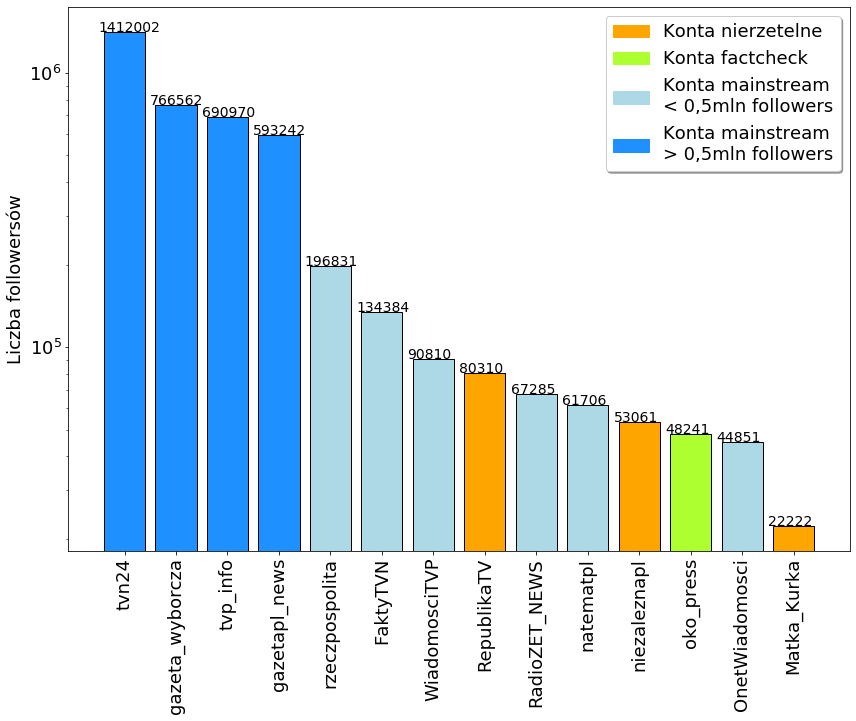
\includegraphics[width=0.9\linewidth]{img/results/followers.png}
	\caption{Wykres liczby followersów najbardziej popularnych kont z\,podziałem na przynależność do klasy}
\end{figure}
\par
W pierwszej dziesiątce najpopularniejszych kont z\,przeprowadzanej analizy (z wyłączeniem Bigmainstream) trzy pozycje zajmują konta oznaczone jako Junk. Z\,tej kategorii najwięcej followersów ma RepublikaTV i\,znajduje się ona na 4 miejscu. Strona z\,kategorii Factcheck znalazła się dopiero na siódmym miejscu w\,popularności.

\subsection{Liczba tweetów}
Konta mediów zakwalifikowanych jako mainstreamowe łącznie opublikowały łącznie 25 tysięcy postów, w\,tym 8 tysięcy postów należy do kont posiadających ponad pół miliona followersów. Natomiast konta Junk opublikowały 10 tysięcy postów. W\,te statystyki wliczają się tweety oryginalnie opublikowane przez te konta jak i\,udostępnione przez nie retweety.  
\par
Sprawdzono, jak duża część zebranych tweetów w\,każdej klasie jest oryginalnie stworzona przez znajdujące się w\,niej konta. Wyniki przedstawiono w\,tabeli \ref{tab:liczbatweetowklasy}. Okazuje się, że największy procent oryginalnych tweetów do wszystkich tweetów publikują konta z\,klasy Nierzetelne. Natomiast najmniej, bo tylko 75\% tweetów publikowanych przez konta mainstream, jest oryginalnie przez nie postowany.
\begin{table} 
\centering 
\caption{Porównanie liczby oryginalnych tweetów do wszystkich tweetów danej klasy.} \label{tab:liczbatweetowklasy}
\begin{tabular}{|m{2,8cm}|R{2,5cm}|R{2,5cm}|R{2,5cm}|R{2,5cm}|} 
\hline
~Klasa & Suma 
  wszystkich & Suma 
  \mbox{oryginalnych} & Procent
  
  oryginalnych & Średnia
  
  oryginalnych
  /dzień \\ 
\hline
NIERZETELNE & 10466 & 10246 & 98\% & 330.5 \\ 
\hline
MAINSTREAM \textless{}
  0,5 mln & 17484 & 12566 & 72\% & 405.4 \\ 
\hline
MAINSTREAM \textgreater{}
  0,5mln & 8078 & 6463 & 80\% & 208.5 \\ 
\hline
FACTCHECK & 644 & 607 & 94\% & 19.6 \\
\hline
\end{tabular}
\end{table}

\subsection{Analiza aktywności kont}
Posiadając informacje na temat oryginalnych tweetów, można było zbadać z\,jak duzo nowych tweetów jest publikowane przez konta w\,każdej klasie. Ogólne dane przedstawiono w\,tabeli \ref{tab:liczbatweetowklasy}. W\,tym przypadku dla lepszego rozeznania zdecydowano się spojrzeć które konta są najbardziej aktywne. Może się bowiem zdarzyć, że w\,zbiorze kont, tylko kilka z\,nich publikuje bardzo duzo treści natomiast inne ograniczają liczbę swoich publikacji. 
\par
\begin{figure}[!h]
	\centering 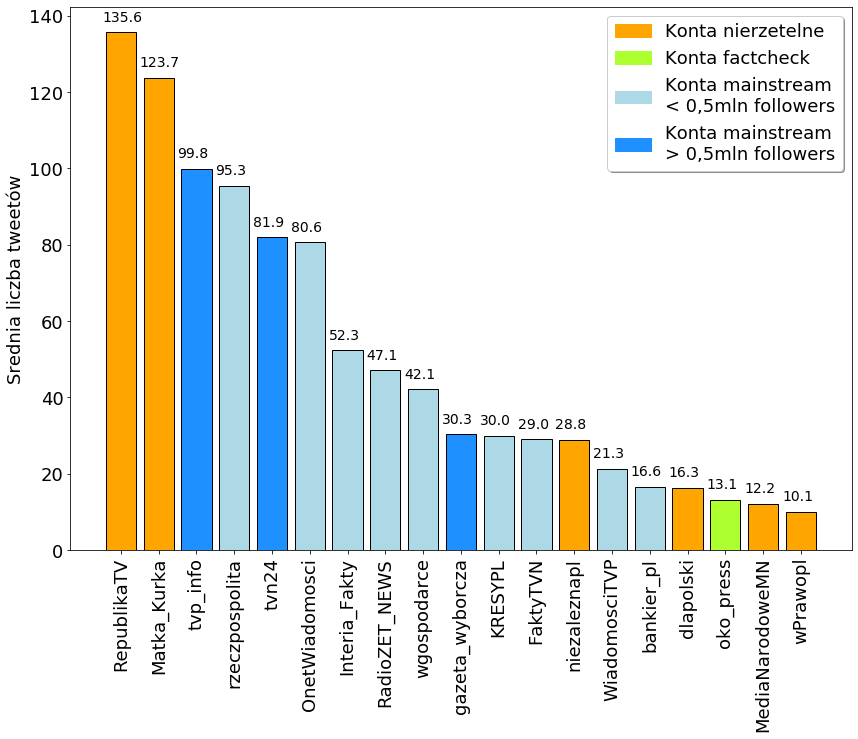
\includegraphics[width=0.9\linewidth]{img/results/tweetsperday.png}
	\caption{Wykres średniej liczby publikowanych oryginalnych tweetów na dzień dla najbardziej aktywnych kont z\,podziałem na przynależność do klasy} \label{fig:tweetsperday}
\end{figure}
\par
Badając liczbę oryginalnych tweetów dla każdego z\,kont stworzono wykres piętnastu najbardziej aktywnych kont. Aktywność liczono jako średnią liczbę oryginalnych postów na dzień. Wyniki przedstawiono w\,wykresie na rysunku \ref{fig:tweetsperday}. Okazuje się, że różnica w\,aktywności kont jest ogromna. Są konta i\,z kategorii nierzetelne oraz z\,kategorii mainstream które publikują średnio po kilkaset oryginalnych postów dziennie. W\,analizowanym zbiorze znajduje się jednak też kilka kont, które są prawie nieaktywne co oznacza, że zebrano dla nich mniej niż 10 tweetów w\,badanym okresie czasu. Dodatkowo dla konta crowdmedia nie istniał żaden post możliwy do pobrania.
\subsection{Analiza korelacji tweetów pomiędzy analizowanymi kontami }
Posiadając zbiór postów analizowanych kont, który zawiera nie tylko posty oryginalnie stworzone przez te konta, ale również retweety postów z\,innych kont, chciano sprawdzić, czy istnieją relacje pomiędzy badanymi kontami. 
\par
Dokonując tej analizy chciano zbadać dwie rzeczy. Pierwszym celem było zbadanie, czy badane konta udostępniają nawzajem swoje tweety, oraz jeśli tak to czy należą one do tej samej klasy czy do różnych klas. Drugim celem było sprawdzenie czy istnieją konta, nie będące uwzględnionymi w\,obecnym zbiorze klasyfikacji, z\,których konta, które znajdują się w\,tym zbiorze udostępniają treści. Dzięki temu planowano wykryć niebezpośrednie relacje pomiędzy badanymi kontami.
\par
Aby ułatwić tę analizę stworzono wizualną reprezentację sieci udostępnień tweetów przez konta (Rysunek \ref{fig:connectedaccounts}). Zawarto w\,niej wszystkie konta ze zbioru klasyfikacji, które udostępniły przynajmniej jeden post opublikowany oryginalnie przez inne konto ze zbioru. Na tym samym rysunku przedstawiono również inne konta, które były udostępnione przynajmniej 30 razy przez któreś z\,badanych kont. 
\par
Na rysunku konta zostały przedstawione jako wierzchołki, zakodowane kolorem w\,zależności od klasy, do której należą. Konta nie należące do żadnej z\,klas zostały opatrzone etykietą ‘Inne’. Należą one do grafu skierowanego, gdzie łuk istnieje między wierzchołkiem A\,a wierzchołkiem B, gdy konto A\,udostępniło post konta B. Na rysunku grubość łuków wyraża jego wagę liczoną jako liczbę udostępnionych postów. Jest to jednak wartość tyko poglądowa, ponieważ skala możliwych wartości była zbyt duża, aby czytelnie odzwierciedlić ją na rysunku. 
\begin{figure}[!h]
	\centering 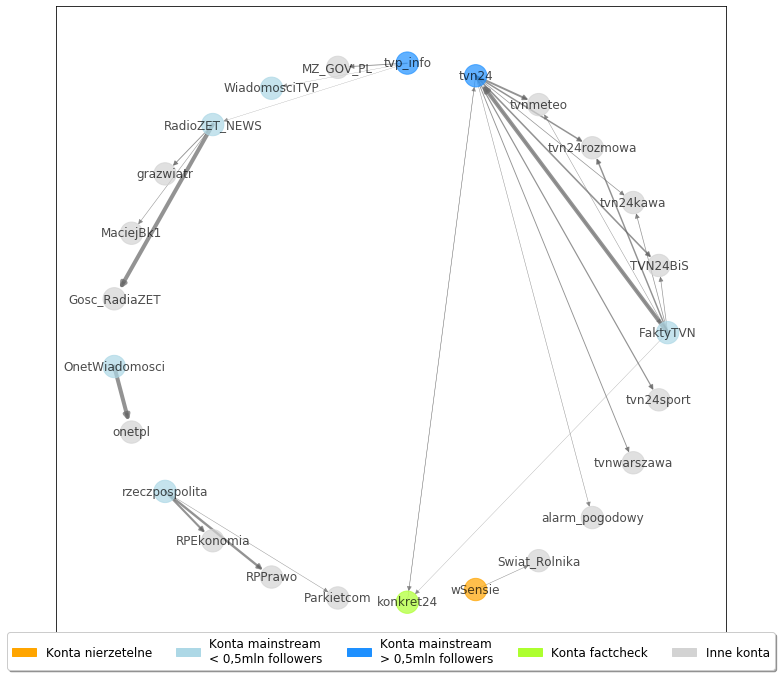
\includegraphics[width=1.0\linewidth]{img/results/connectionbetweenaccounts.png}
	\caption{Sieć udostępnień tweetów przez konta z\,podziałem na  klasy} \label{fig:connectedaccounts}
\end{figure}
\par
Dzięki stworzonemu rysunkowi, przedstawiającemu sieć udostępnień tweetów pomiędzy znaczącymi kontami można zauważyć, że generalnie nie ma zbyt wiele relacji pomiędzy analizowanymi kontami. Na 28 kont, w\,prezentowanej sieci znalazło się tylko 10 z\,nich. Co można zauważyć, to fakt, że najczęściej udostępniane są treści należące do tej samej grupy wydawniczej. Najlepszym przykładem tutaj jest grupa TVN, gdzie na koncie tvn24 oraz FaktyTVN udostępniane są posty z\,siostrzanych serwisów należących do tej samej grupy. To samo zjawisko występuje również dla pozostałych kont. 
\subsection{Analiza udostępnianych domen }
W kolejnym badaniu chciano sprawdzić jakie zewnętrzne serwisy są udostępniane przez analizowane konta. Celem, podobnie jak w\,badaniu powyżej, było sprawdzenie czy istnieją relacje między badanymi kontami. W\,tym przypadku chciano zbadać, czy istnieją takie wspólne domeny, które są udostępniane przez analizowane konta, i\,jeśli tak to czy te konta należą do jednej klasy czy różnych.
W celu analizy takich zależności pobrano wszystkie linki url które znajdowały się w\,publikowanych przez badane konta postach. Aby ujednolicić 39 tysięcy pobranych url, skupiono się jedynie na domenach do których te linki prowadzą. Dodatkowo najpierw należało rozszerzyć niektóre z\,linków, ponieważ duża część z\,nich była poddana działaniu serwisów skrócających url. 
\par
Z pobranych danych stworzono graf dwudzielny, gdzie pierwszym zbiorem są analizowane konta a\,drugim domeny przez nie udostępniane w\,postach. Aby domena znalazła się w\,tym zbiorze musiała być udostępniona przez jakieś konto przynajmniej 30 razy w\,analizowanym zbiorze. Łuk istnieje między nimi, gdy konto udostępniało w\,swoich postach daną domenę. 
\begin{figure}[!h]
	\centering 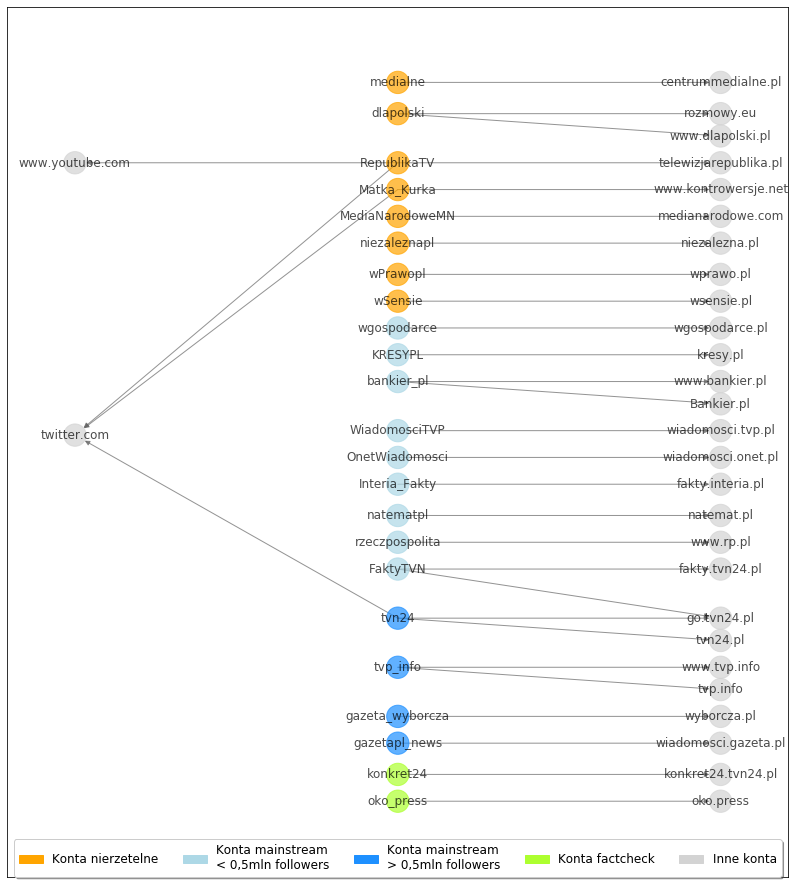
\includegraphics[width=1.0\linewidth]{img/results/connectionwithlikns.png}
	\caption{Sieć udostępnień domen przez konta z\,podziałem na klasy} \label{fig:connectedlinks}
\end{figure}
Dzięki wizualizacji grafu ukazującego udostępnienia domen przez analizowane konta \ref{fig:connectedlinks} można łatwo zobaczyć, że udostępnianie zewnętrznych domen w\,postach na tweeterze w\,omawianym przypadku sprowadza się prawie wyłącznie do udostępniania serwisu, do którego to konto należy. Jedyną domeną która jest udostępniana przez kilka kont jest twitter.com, znajdują się tam linki do innych tweetów, których zapewne nie chciano bezpośrednio udostępnić. 
\subsection{Ilość bezpośrednich udostępnień }
Do tej analizy wzięto pod uwagę jedynie oryginalne posty, ponieważ mimo że na popularność tweeta ma znaczenie kto go udostępnił, bo to zapewnia większą grupę odbiorców, to popularność postu nie wpływa na statystykę popularności użytkowników, którzy dokonali dalszego udostępnienia. 
\par
Konta oznaczone jako factcheck publikują stosunkowo mało postów w\,porównaniu do innych klas. Jednak te posty cieszą się dużą popularnością, jeśli chodzi o dalsze ich udostępnienie. Średnio post ma 18 retweetów, dzięki czemu 600 tweetów zostało powielone 11 tysięcy razy. Posty publikowane przez największe mainstremowe media nazywane tu Bigmainstream są średnio udostępniane przez 10 użytkowników. Ten wynik nie dziwi biorąc pod uwagę jak dużo osób obserwuje te konta.  
\par
Co ciekawe można zauważyć, że oryginalne posty mainstremowe w\,tym przedziale czasowym były udostępniane dalej przez średnio 2.9 użytkowników, czyli łącznie były udostępnione prawie 36 tysięcy razy. Średnia liczba retweetów posta opublikowanego przez Junk accounts wynosi 7.1 co oznacza ze te posty łącznie były udostępnione prawie 73\,tysięcy razy. Jest to dwa razy więcej niż łączna ilość udostępnień postów mainstreamowych mimo że postów mainstreamowych było 20 procent więcej oraz posiadają one łącznie trzy razy więcej followersów. 


\begin{table}[!h]
\centering
\caption{Porównanie liczby retweetów zebrancyh tweetów z podziałem na klasy.} \label{tab:liczbaretweetow}
\begin{tabular}{|m{2,8cm}|R{2,5cm}|R{2,5cm}|R{2,5cm}|}  
\hline
~Klasa & Liczba tweetów & Łączna liczba retweetów & Średnia liczba retweetów na tweet \\ 
\hline
NIERZETELNE & 10246 & 72975 & 7.1 \\ 
\hline
MAINSTREAM \textless{} 0,5 mln & 12566 & 35965 & 2.9 \\ 
\hline
MAINSTREAM \textgreater{} 0,5mln & 6463 & 61156 & 9.5 \\ 
\hline
FACTCHECK & 607 & 11020 & 18.2 \\
\hline
\end{tabular}
\end{table}

\subsubsection{Zróżnicowanie popularności kont}
Poniżej przedstawiono dwa wykresy omawiające w\,większych szczegółach charakterystykę udostępnień postów. Pierwszy z\,wykresów pokazuje średnią liczbę udostępnień oryginalnych postów dla najbardziej popularnych kont. Popularność konta oznacza tu liczbę udostępnień jakie otrzymują jego posty. Można też ją określić jako aktywność odbiorców. Jak widać na rysunku \ref{fig:retweets-per-tweet} popularność konta nie zależy od klasy do której należy i\,jest zróżnicowana w\,każdej klasie.
\begin{figure}[!h]
	\centering 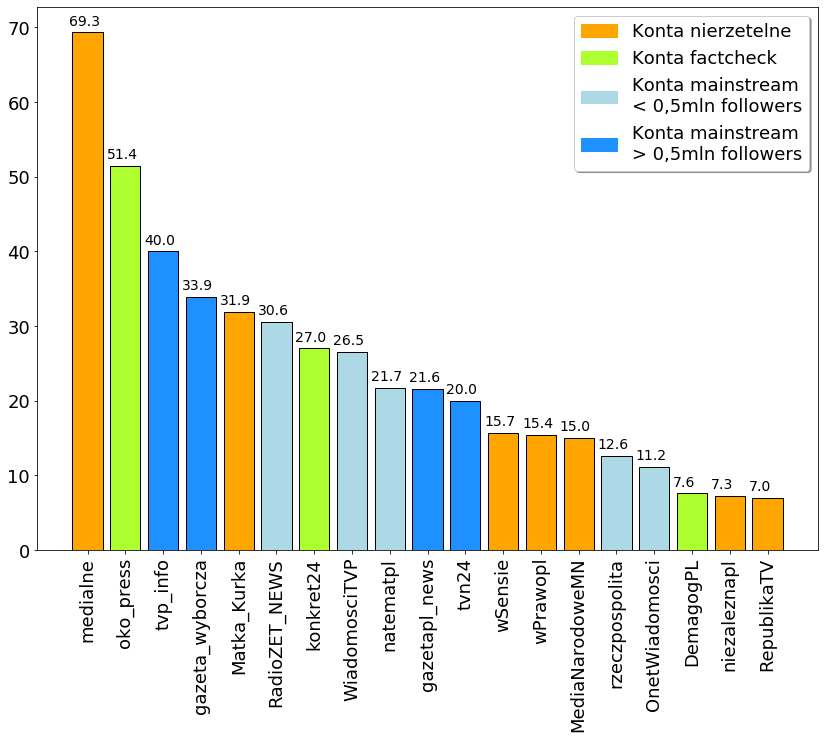
\includegraphics[width=0.95\linewidth]{img/results/retweetspertweet.png}
	\caption{Wykres średniej liczby udostępnień oryginalnych tweetów dla najbardziej popularnych kont z\,podziałem na przynależność do klasy.} \label{fig:retweets-per-tweet}
\end{figure}

\subsubsection{Liczba followers a\,popularność kont}
Następnie chciano zbadać czy na popularność treści publikowanych przez konta wpływa liczba jego subskrybentów. W\,tym celu stworzono wykres dwuwymiarowy w\,którym na osi x podano liczbę followers w\,skali logarytmicznej. Natomiast na osi y zaznaczono średnią liczbę udostępnień jaką otrzymują posty. Dodatkowo wielkością punktu na wykresie oznaczono aktywność konta liczoną jako średnia liczba postów publikowanych w\,czasie dnia. Wszystkie punkty zostały również oznaczone odpowiednim kolorem, w\,zależności, do której klasy należą. Zrezygnowano z\,nadania im nazw kont ze względu na czytelność wykresu, zwłaszcza, że w\,przypadku tego badania nie ma to większego znaczenia. 
\begin{figure}[!h]
	\centering 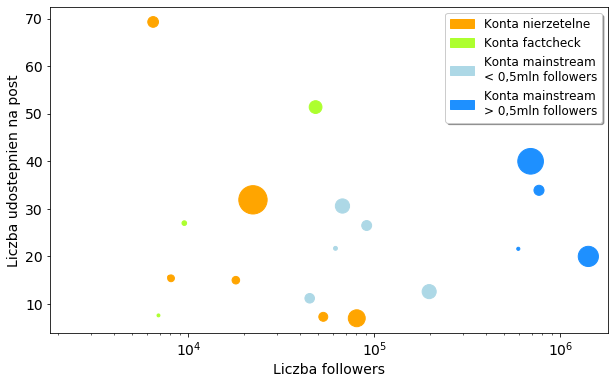
\includegraphics[width=0.95\linewidth]{img/results/retweetsvsfollowers.png}
	\caption{Średnia liczba udostępnień posta a\,liczba followersów dla kont z\,podziałem na klasy.} \label{fig:retweets-vs-followers}
\end{figure}
\par

Na podstawie stworzonego wykresu można wyciągnąć wnioski, że ani liczba subskrybentów konta ani częstość publikacji nowych treści nie ma wyraźnie większego wpływu na aktywność odbiorców w\,liczbie udostępnień postów. Dwa konta o\,liczbie followersów większej niż pół miliona posiadają jedne z\,najwyższych popularności w\,tym zbiorze, jednak w\,tej klasyfikacji wyraźnie przewyższają je konta posiadające 10 razy mniejszą grupę odbiorców.  Podobnie nie widać żadnego schematu, aby odpowiednia liczba publikowanych postów w\,czasie dnia wpływała pozytywnie na aktywność odbiorców tych postów. 


\subsection{Użytkownicy udostępniający}
Następnym krokiem analizy kont, było dokonanie badania użytkowników udostępniających posty. Jak powiedziano wcześniej, analiza nie będzie dotyczyła szczegółów użytkowników ze względu na ich prywatność. Skupiono się jedynie na ich zachowaniu względem analizowanych kont. Łącznie dla 15 tysięcy postów pobrano 11 tysięcy unikalnych użytkowników. Stworzono analizę, badającą średnie zachowanie tych użytkowników. Należy jednak zaznaczyć, że są to grupy użytkowników udostępniający posty danej klasy, ale nie oznacza to, że wyłącznie tej jednej klasy. 
\par
Najbardziej aktywnymi użytkownikami są Ci udostępniający posty kont oznaczonych jako nierzetelne. Średnio użytkownik z\,tej grupy udostępnił 10 postów ze zbioru zebranych nierzetelnych postów. Dla porównania średnia liczba udostępnień przez użytkownika postów typu mainstream to niecałe 5 postów.  Użytkownik, który dokonał maksymalnej liczby udostępnień wśród zebranych postów udostępnił 1900 tweetów z\,klasy nierzetelne. 


\begin{table}[!h]
\centering 
\caption{Porównanie liczby oryginalnych tweetów do wszystkich tweetów danej klasy.} \label{tab:liczbaretweeterow}
\begin{tabular}{|m{2,8cm}|R{2,5cm}|R{2,5cm}|R{2,5cm}|R{2,5cm}|} 
\hline
Klasa kont & Liczba tweetów & Unikalni użytkownicy & Max udostępnienia /użytkownika & Średnio udostępnienia/ użytkownika \\ 
\hline
JUNK & 5685 & 4217 & 1962 & 9.9 \\ 
\hline
MAINSTREAM \textless{} 0,5mln & 5539 & 5311 & 842 & 4.0 \\ 
\hline
MAINSTREAM \textgreater{} 0,5mln & 4425 & 6718 & 1019 & 5.2 \\ 
\hline
FACTCHECK & 384 & 1994 & 67 & 2.9 \\
\hline
\end{tabular}
\end{table}

\subsubsection{Aktywność użytkowników udostępniających}
Dla wszystkich klas łącznie średnia liczba udostępnień przez użytkownika wynosi 6\,ale mediana wynosi już tylko 2 posty na użytkownika. Na rysunku \ref{fig:retweets-per-user} przedstawiono wykresy kołowe ukazujące jaki procent użytkowników udostępnił określoną liczbę postów z\,danej klasy. 
\begin{figure}[!h]
	\centering 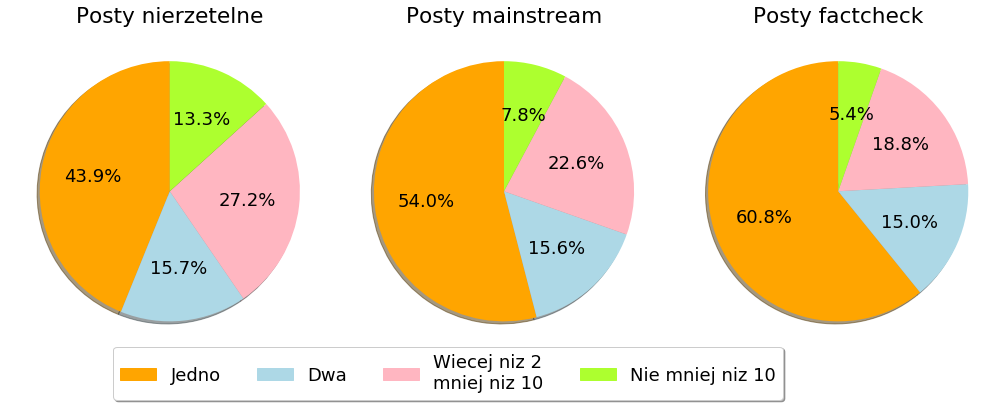
\includegraphics[width=0.9\linewidth]{img/results/retweetsperuser.png}
	\caption{Procent użytkowników z\,określoną liczbą udostępnień postów z\,danej klasy.} \label{fig:retweets-per-user}
\end{figure}

\par
Dzięki rysunkowi wyraźnie widać, że ponad połowa użytkowników udostępniła maksymalnie dwa posty ze zbioru z\,każdej klasy. Tylko niewielki procent użytkowników udostępniał nie mniej niż 10 postów z\,danej klasy. Jednak największy procent takich użytkowników należy do klasy postów nierzetelnych. Dodatkowo ciekawym jest, że ponad 45\% wszystkich użytkowników udostępniło tylko jeden post gdy brano pod uwagę wszystkie posty niezależnie od klasy do której należą.


\subsection{Wnioski z analizy}
Celem przeprowadzonej analizy było zbadanie charakterystyk kont, treści przez nie publikowanych oraz ich odbiorców. W części badań skupiano się na właściwościach wszystkich kont w danej klasie aby przeprowadzić całościową analizę porównawczą charakterystyk przedstawianych klas. Porównywano trzy klasy: konta nierzetelne, mainstream oraz factcheck. Z powodu dużej różnicy w ilości tzw. followersów, czyli odbiorców kont mainstream zdecydowano wyróżnić w śród tych kont dwa niezależne niepokrywające się podzbiory. Granicę ustalono na 0,5 mln followersów. Okazało się być to dobrym wyborem ponieważ kolejna największa liczba followersów to 0,2 mln.  
\par Różnicę w ilości odbiorców widać patrząc na średnią liczbę udostępnień postów przez użytkowników. Konta mainstream o dużej liczbie followersów posiadają średnio więcej udostępnień, niż te z mniejszą liczbą. Różnicę widać również w liczbie publikowanych nowych postów. Liczba postów oraz followersów niekoniecznie jednak wpływa bezpośrednio na liczbę udostępnień. Konta należące do serwisów factcheck mimo posiadania stosunkowo małej liczby followersów otrzymują średnio najwięcej udostępnień ze wszystkich grup.
\par
Zbadano również zachowania użytkowników udostępniających posty. Okazuje się, że prawie połowa zebranych użytkowników udostępniła tylko i wyłącznie jeden post. Najbardziej aktywnymi, pod względem liczby udostępnień, użytkownikami są użytkownicy udostępniający posty kont kategorii nierzetelne.
\par
Dodatkowo zbadano połączenia pomiędzy kontami, w formie wzajemnych udostępnień swoich postów. Chciano w ten sposób sprawdzić czy istnieją bezpośrednie lub niebezpośrednie zależności między nimi w utworzonych klasach lub pomiędzy nimi. Okazuje się jednak, że takie połączenia istnieją jedynie pomiędzy kontami należącymi do tego samego wydawcy. Oznacza to, że badane konta zazwyczaj nie udostępniają informacji pochodzących z innych źródeł. Największy procent oryginalnych treści posiadają konta z\,kategorii nierzetelne.  Zbadano również, jakie domeny są linkowane w postach badanych kont, i podobnie okazuje się, że konta linkują informacje jedynie z serwisów do których należą. 
\par
Po tej analizie widać, że najbardziej obiecującą właściwością charakteryzującą konta w poszczególnych klasach mogą być użytkownicy którzy udostępniają ich posty. Mimo, że połowa użytkowników udostępnia około 2 posty to istnieje  nadal niemała grupa osób która udostępnia ich bardzo dużo. Na tej podstawie można próbować klasyfikacji postów. Należy zobaczyć jak duża grupa osób jest spolaryzowana na konkretną klasą postów, oraz jak dużo osób udostępnia posty pochodzące z kont zaklasyfikowanych do różnych klas. Mając te informacje można potraktować użytkowników udostępniających posty jako charakterystykę kont. Można badać prawdopodobieństwo preferencji użytkowników lub posiadając wiedzę o użytkownikach przewidywać prawdopodobieństwo przynależności informacji do konkretnej klasy. 
\newpage
\section{Klasyfikacja informacji publikowanych w\,social media}
W poniższym rozdziale opisano przebieg i\,wyniki klasyfikacji postów pobranych z\,Twee- tera pod względem przynależności do jednej z\,dwóch klas. Badania te oparto na pracy Some Like it Hoax\cite{tacchini2017some} w\,której przeprowadzono klasyfikację postów pobranych z\,platformy facebook otrzymawszy bardzo wysoką precyzję. Celem badań w\,obecnej pracy jest sprawdzenie możliwości klasyfikacji postów z\,zebranego zbioru polskojęzycznego. Klasyfikacja będzie dokonywana na podstawie informacji o\,udostępnieniach tych postów przez użytkowników. Dodatkowym celem jest sprawdzenie jak duży musi być zbiór zaklasyfikowanych danych podany jako zbiór uczący, aby otrzymać zadowalającą precyzję klasyfikacji.
\subsection{Opis badań Some Like It Hoax}
Badania w\,pracy Some Like it Hoax opierano na postach publikowanych przez wybrane konta na platformie Facebook. Konta te były zaklasyfikowane do odpowiedniej z\,dwóch klas. Dla wszystkich postów pobrano również informacje, o\,osobach które ten post polubiły. Używając tych danych przeprowadzono klasyfikację przy pomocy algorytmu regresji logistycznej oraz autorskiej modyfikacji algorytmu traktując problem tej klasyfikacji jak problem binarnego etykietowania poprzez crowsourcing (eng. boolean label crowdsourcing).
Wykorzystując fakt, że większość użytkowników ograniczała swoją aktywność tyko do postów należących do tylko jednej z\,tych kategorii, ale istnieje też niemała grupa akceptująca oba rodzaje stron możliwe było osiągnięcie bardzo wysokich wyników klasyfikacji postów do odpowiedniej kategorii. Jednak również wykorzystując grupy użytkowników niespolaryzowanych możliwe było rozpoznanie klasy posta z\,wysokim prawdopodobieństwem.
\subsubsection{Opis wyników badań}
Do badań w\,2017 roku pobrano 15,500 postów polubionych 2 miliony razy przez ponad 900 tysięcy użytkowników. Dla obu użytych algorytmów przeprowadzano badania dla dwóch zbiorów danych z\,różniącymi się wskaźnikami. Były nimi zbiór wszystkich postów wraz ze wszystkimi użytkownikami. Oraz zbiór postów polubionych przez użytkowników, którzy polubili posty z\,obu klas nazwany zbiorem intersekcji. W\,trakcie badań udało się twórcom uzyskać bardzo wysokie wyniki. 
\par
Najwyższe wyniki uzyskano dla algorytmu harmonicznego traktującego cały zbiór danych jako zmodyfikowany problem etykietowania. Dla takiego zestawienia uzyskiwano prawie perfekcyjną dokładność 99,4\% nawet gdy w\,zbiorze trenującym znajdowało się 0,5\% danych, czyli 80postów
W przypadku tylko zbioru intersekcji nieznacznie lepsza okazała się być metoda regresji logistycznej. Uzyskano precyzję na poziomie 90\% przy wykorzystaniu 10\% zbioru do nauki modelu. 
\par 
Poniżej na rysunku \ref{fig:wyniki-somelikeithoax} załączono wykres prezentujący całościowe wyniki tej pracy. Przedstawia on wyniki precyzji na osi y względem wielkości zbioru uczącego wyrażonego w jego stosunku do wielkości całego zbioru. Na tym wykresie pokazano cztery serie danych po dwie dla każdego z zbiorów danych dla każdego z algorytmów: regresji logistycznej oraz algorytmu harmonicznego.

\begin{figure}[!h]
	
	\centering 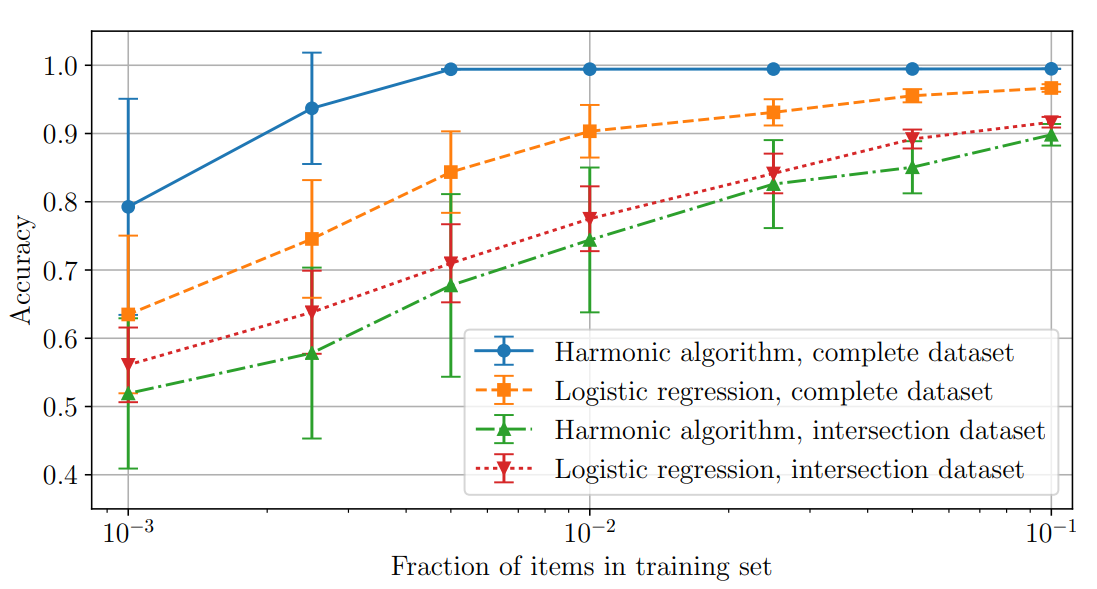
\includegraphics[width=0.9\linewidth]{img/results/wyniki-somelikeithoax.png}
	\caption{Wyniki badań klasyfikacji postów pochodzących z platformy Facebook. Źródło:\cite{tacchini2017some}}\label{fig:wyniki-somelikeithoax}
\end{figure}

\subsection{Opis odtworzenia badań }
Ze względu na niedostępność danych z\,platformy Facebook, musiało nastąpić kilka przekształceń w\,odtwarzaniu badań klasyfikacji nierzetelnych informacji na podstawie pracy Some Like It Hoax. Jednak mimo zmiany źródła pobierania danych logika pozostała niezmieniona. Na podstawie odkryć innych badań otrzymano listę kont należących do kilku kategorii. Sposób utworzenia listy danych opisano w\,podrozdziale \ref{wybor-danych}. Do tego badania ograniczono się do kategorii Junk odpowiadającej kategorii Hoax oraz kategorii Mainstream odpowiadającej kategorii Non-hoax. Dla odpowiednich kont na twitterze pobrano publikowane przez nie posty oraz informacje, o\,użytkownikach które ten post retweetowały czyli udostępniły na swoim koncie. 
\par
Aby jednak w\,dalszej części badań zachować jak największą spójność do odtworzenia wyników klasyfikacji dla obecnie analizowanych danych użyto udostępnionego kodu stworzonego przez twórców pracy Some Like It Hoax. 

\subsection{Opis użytych algorytmów }
Dokonano dwa podejścia do rozwiązania problemu klasyfikacji postów. Jako pierwsze potraktowano ten problem jako nadzorowaną klasyfikacje binarną używając regresji logistycznej. Następie przedstawiono ten problem jako problem binarnego etykietowania poprzez crowdsourcing (ang. boolean label crowdsourcing problem BLC). 
\subsubsection{Regresja logistyczna}
Przedstawiając powyższy problem jako nadzorowaną klasyfikację binarną klasyfikujemy przynależność postów do odpowiedniej z\,dwóch klas – Junk albo Mainstream. Dzieje się to na podstawie ich cech, w\,tym przypadku cechami są użytkownicy. Każdy post posiada zbiór cech, który może przyjmować jedną z\,dwóch możliwych wartości – 1, gdy dany użytkownik udostępnił dany post lub 0, gdy dany użytkownik nie udostępnił danego postu.
\par
Regresja logistyczna polega na wyuczeniu modelu poprzez znalezienie odpowiednich wag dla cech modelu.  W\,przedstawianym modelu są to wagi użytkowników. W\,praktyce waga większa od zera oznacza, że użytkownik udostępnia w\,większości posty mainstreamowe a\,waga mniejsza od zera oznacza, że użytkownik udostępnia w\,większości posty należące do kategorii Junk. Na podstawie wyuczonych wag model oblicza prawdopodobieństwo, że post należy do klasy mainstream.

\subsubsection{Binarne etykietowanie poprzez crowdsourcing}
Drugim podejściem jest przedstawienie problemu klasyfikacji postów jako problemu etykietowania poprzez crowdsourcing, czyli poprzez niepowiązane ze sobą osoby. Ten rodzaj problemów opisuje sytuacje w\,której duża grupa użytkowników oznacza dane etykietami prawda lub fałsz. Taka metoda może być używana do oznaczania czy edycja postu na Wikipedii jest aktem wandalizmu lub czy post lub strona jest odpowiednia dla dzieci\cite{de2015reliable}. W\,kontekście analizowanego zbioru postów na Twitterze uznano udostępnienie postu przez użytkownika jako oznaczenie go etykietą ‘prawda’.
\par
Badany problem różni się jednak nieznacznie od binarnego etykietowania poprzez crowdsourcing. Albowiem w\,BLC zakłada się, że użytkownicy dokonujący etykietowania są bardziej skłonni mówić prawdę. Algorytmy rozwiązujące ten problem porównują etykiety nadane przez użytkowników i\,naprostowują wyniki biorąc pod uwagę możliwość kłamstwa, aby uzyskać wyniki jakie etykiety powinny być posiadać obiekty.  Dlatego też nie jest tam używany zbiór uczący do dokonywania nadzoru.
\par
Natomiast w\,przypadku nadawania etykiet kategorii postom na Twitterze nie możemy zakładać, że użytkownicy będą preferowali udostępnianie postów mainstreamowych nad tymi z\,kategorii Junk. Co więcej, dzięki wcześniejszej analizie danych w\,rozdziale 8.5, wiemy że posty z\,obu kategorii mają porównywalną łączną liczbę udostępnień. Biorąc to więc pod uwagę należy posługiwać się zbiorem uczącym z\,określoną etykietą klasy.
\subsubsection{Algorytm harmoniczny}
Do podejścia przedstawiającego problem klasyfikacji postów jako problem BLC użyto algorytmu harmonicznego zaadaptowanego do tego zadania przez twórców pracy Some Like It Hoax. Algorytm ten opiera się na algorytmie przedstawionym dwa lata wcześniej\cite{de2015reliable} ale został dostosowany do dokonania klasyfikacji z\,zastosowaniem zbioru uczącego. 
\par
	Zbiór danych przedstawiony jest jako graf dwudzielny, gdzie wierzchołkami są posty oraz użytkownicy a\,łukami są zaznaczone udostępnienia postów przez użytkowników.  Bezpośrednie sąsiedztwo wierzchołków oznacza, że między postem a\,użytkownikiem nastąpiła interakcja.
\par
Traktując część postów jako zbiór uczący nadano im odpowiednie współczynniki, resztę pozostawiając nieokreśloną. Dzięki temu zabiegowi algorytm jest wstanie w\,pierw- szym kroku obliczyć prawdopodobieństwo upodobań użytkowników, którzy te posty udostępnili. W\,praktyce oznacza to prawdopodobieństwo preferowania postów z\,kategorii Junk lub Mainstream. Aby uznać, że użytkownik jest spolaryzowany na daną kategorię musi posiadać on przewagę 2:1 udostępnień dla jednej z\,kategorii. 
\par
	Posiadając te informacje w\,kolejnych krokach zostają uaktualnione współczynniki postom które nie należą do zbioru uczącego a\,były udostępnione przez użytkowników o\,znanych już preferencjach. Następnie zostają uaktualnione preferencje użytkowników będących w\,bezpośrednim sąsiedztwie do postów posiadających etykiety. Dzięki kilkukrotnej iteracji tych kroków wiedza na temat postów oraz preferencji użytkowników zostaje rozpropagowana wewnątrz grafu. Taka możliwość transmisji informacji w\,grafie daje perspektywy na uzyskanie wysokich wyników precyzji klasyfikacji nawet z\,małego zbioru zaklasyfikowanych postów na początku algorytmu.

\subsection{Opis przygotowania danych }
Do badań klasyfikacji postów pobrano 21950 tweetów z\,okresu 22.03-10.04.2020. Posty te są zaklasyfikowane do odpowiedniej z\,dwóch klas, Nierzetelne lub Mainstream, w\,zależności od przynależności do klasyfikacji konta, z\,którego pochodzą. Jednak do przeprowadzenia automatycznej klasyfikacji możliwe jest użycie jedynie tych postów które posiadają przynajmniej jedno udostępnienie. Takich postów pobrano 15529.  Wśród nich otrzymano 5563 postów pochodzących z\,kont Nierzetelnych oraz 9966 postów z\,kont Mainstream. Sumując wszystkie zebrane udostępnienia zebrano ich łącznie prawie 100 tysięcy. W\,tym 41 tys. oraz 56 tys. odpowiednio dla kont z\,powyższych kategorii. Zestawienie danych można znaleźć w\,tabeli \ref{tab:zbiordanych} zamieszczonej poniżej.
\begin{table}[!h]
\centering
\caption{Analiza zebranych danych do przeprowadzenia klasyfikacji.} \label{tab:zbiordanych}
\begin{tabular}{|m{4cm}|R{2,5cm}|R{2,5cm}|R{2,5cm}|} 
\hline
~ & Wszystkie & Nierzetelne & Mainstream \\ 
\hline
Liczba wszystkich zebranych tweetów & 21950 & 7605 & 14345 \\ 
\hline
Tweety udostępnione przynajmniej raz & 15524 & 5560 & 9964 \\ 
\hline
Liczba udostępnień & 97820 & 41102 & 56718 \\ 
\hline
Unikalni \mbox{udostępniający} & 11477 & 2031 & 7287 \\
\hline
\end{tabular}
\end{table}
\par
Dla opisanych wyżej danych udało się pobrać informacje o\,11 tysiącach unikalnych użytkownikach. W\,tym można zauważyć, że około 60\% tych użytkowników dokonywało udostępnienia tylko postów należących do kont mainstreamowch. Dwa tysiące osób udostępniało wyłącznie posty publikowane przez konta okreslone w\,tej pracy jako Nierzetelne. Natomiast tylko niewiele więcej użytkowników udostępniało posty obu klas kont.  
\subsubsection{Opis używanych zbiorów danych}
Na podstawie tych zebranych danych stworzono dwa zbiory służące do przeprowadzania algorytmów klasyfikacji. Pierwszym z\,nich jest zbiór zawierający wszystkie posty które były udostępnione przynajmniej raz, będzie on nazywany zbiorem pełnym. Zawiera on obiekty którymi są posty wraz z\,listą wszystkich użytkowników którzy go udostępnili. Zbiór ten ma wielkość 12 tysięcy postów.
\par
Drugi zbiór jest podzbiorem pierwszego, ale opiera się na założeniu wykorzystnia tylko takich użytkowników którzy udostępnili przynajmniej jeden post z\,klasy nierzetelny i\,przynajmniej jeden post z\,klasy mainstream. Jest więc to zbiór zawierający tylko te posty, które były udostępnione przez powyżej opisanych użytkowników. Zawiera on 12 tys. postów udostępnionych 54 tys. razy przez 2159 unikalnych użytkowników. Będzie on nazywany zbiorem intersekcji, z\,powodu pochodzenia zbioru użytkowników.
\par
Analizę porównawczą zbioru pełnego oraz zbioru intersekcji przedstawiono w\,tabeli\,\ref{tab:zbiorydanychklasyfikacja}.
\begin{table}[!h]
\centering
\caption{Tabela porównawcza zbiorów danych poddanych klasyfikacji.} \label{tab:zbiorydanychklasyfikacja}
\begin{tabular}{|m{4cm}|R{2,5cm}|R{2,5cm}|} 
\hline
~ & Zbiór pełny & Zbiór \mbox{intersekcji} \\ 
\hline
Liczba tweetów & 15524 & 12442 \\ 
\hline
Udostępnienia \mbox{tweetów} & 97820 & 54318 \\ 
\hline
Unikalni  \mbox{udostępniający} & 11477 & 2159 \\
\hline
\end{tabular}
\end{table}
\subsection{Opis przeprowadzonych badań}
W poniższym podrozdziale zostaną przedstawione i opisane zaplanowane badania jakie będą przeprowadzone w kolejnym podrozdziale. Ma to na celu przybliżenie metodyki badań, sposobu przeprowadzenia ich oraz opis w jaki sposób pozwolą one osiągnąć odpowiedzi na zaplanowane wcześniej cele.
\subsubsection{Precyzja modelu}
Na obu przygotowanych zbiorach przeprowadzono kilka eksperymentów. Głównym celem było sprawdzenie z\,jaką dokładnością można klasyfikować tego typu dane oraz który z\,algorytmów daje najlepsze wyniki dla określonych zbiorów. Do tego celu zostanie wykorzystana 5-krotna walidacja krzyżowa (ang. 5-fold validation) polegająca na pięciokrotnym sprawdzeniu modelu przy zbiorze uczącym składającym się z\,80\% losowo wybranych danych. 
\subsubsection{Wielkość zbioru uczącego a\,precyzja}
Celem drugorzędnym było sprawdzenie jak duży musi być zbiór uczący, aby otrzymać zadowalające wyniki. W\,przypadku zastosowania automatycznej klasyfikacji postów w\,rzeczywistym systemie jest to bardzo ważna kwestia. Odpowiednie zaklasyfikowanie postów jest zadaniem bardzo kosztownym. Chcąc wykorzystać automatyczną klasyfikację poza środowiskiem badawczym należy wiedzieć czy można takie rozwiązanie skalować na zbiory testowe dużo większe od zbiorów uczących. 
\par
Dla każdej z\,wielkości zbiorów uczących zostanie dokonane 50 powtórzeń algorytmu z\,różnymi danymi w\,zbiorze uczącym. Jako precyzja zostanie pokazana średnia tych 50 powtórzeń. Natomiast prezentowane odchylenie standardowe będzie dotyczyło różnic w\,precyzji pomiędzy przeprowadzonymi powtórzeniami. Zastosowano takie podejście, ponieważ skuteczność nauki modelu klasyfikacji w\,głównej mierze zależy od dostosowania jego zbioru uczącego do zbioru testowego. Mogą się zdarzyć przypadki bardzo o\,bardzo wysokiej precyzji, ale nie świadczy to o\,sukcesie modelu, jeśli pozostałe przypadki rozłożenia danych będą otrzymywały bardzo niskie wyniki.
\par
Podział zbioru na część uczącą i\,testową będzie dokonany semi-logarytmicznie. Zostanie zbadane osiem różnych wielkości zbioru uczącego.  Podział zbioru dokonywany jest w\,taki sposób, że określona część danych zostanie potraktowana jako zbiór uczący, natomiast cała pozostała część zbioru będzie służyła zbadaniu precyzji nauczonego modelu jako zbiór testowy. Celem jest zobaczenie, jak mała część zbioru poddanego klasyfikacji musi mieć znane etykiety, aby automatyczna klasyfikacja miała sens, dając zadowalającą precyzję klasyfikacji nieznanych danych.
\subsubsection{Transmisja wiedzy w\,modelu}
Z tym związana jest również kwestia przenoszenia wiedzy uzyskanej o\,grupie postów na posty pochodzące z\,innych kont. Należy sprawdzić czy, dzięki udostępnieniom użytkowników, system klasyfikacji jest w\,stanie poprawnie nadać etykiety postom z\,innego konta niż zawarte w\,zbiorze uczącym. W\,tym celu zostaną przeprowadzone dwa eksperymenty. W\,pierwszym z\,nich do zbioru uczącego zostaną podane wszystkie posty oprócz postów należących do jednego konta. Taki test zostanie przeprowadzony dla wszystkich możliwych kont. Oraz w\,drugim eksperymencie do zbioru uczącego zostanie podana tylko połowa kont, a\,druga połowa pozostanie w\,zbiorze testowym i\,tak dla wszystkich możliwych kombinacji.
\subsection{Wyniki przeprowadzonych badań}
Poniżej zostaną przedstawione i omówione wyniki otrzymane z przeprowadzonych badań. Kolejne badania zostaną przedstawione w takiej kolejności w jakiej były opisane w podrozdziale wyżej. 
\subsubsection{Precyzja modelu - walidacja krzyżowa}
Pierwszym eksperymentem, który wykonano była 5-krotna walidacja krzyżowa z\,zasto- sowaniem regresji logistycznej, gdzie do każdej iteracji podano 80\% danych do zbioru uczącego. Taka metoda dała zadowalająco wysokie wyniki. Dla zbioru pełnego precyzja wyniosła 0,94\,przy prawie nieznaczącym odchyleniu wynoszącym 0.001. Dla zbioru intersekcji wynik był niewiele słabszy, otrzymawszy precyzję 0.91. 
\par
	Dla algorytmu harmonicznego uzyskano precyzję 0.92 dla zbioru pełnego i\,0.89 dla zbioru intersekcji. Przy wszystkich wynikach odchylenie standardowe było nieznacząco małe. Pełne wyniki tego eksperymentu znajdują się w\,tabeli poniżej Tabela 10 Wyniki klasyfikacji krzyżowej 
\par
Na podstawie tego badania można założyć, że przeprowadzenie automatycznej klasyfikacji na zbiorze składającym się z\,postów i\,użytkowników ich udostępniających jest możliwe.  Największą precyzję przy zachowaniu nieznacząco małego odchylenia standardowego uzyskała metoda regresji liniowej wykonana na pełnym zbiorze. Okazuje się również, że przeprowadzenie regresji liniowej na zbiorze intersekcji jest równie dobrym sposobem klasyfikacji jak przeprowadzenie algorytmu harmonicznego na pełnym zbiorze. Jednak, aby zobaczyć jak te algorytmy zachowują się dla różnych wielkości zbiorów danych uczących w\,stosunku do danych testowych zostaną przeprowadzone kolejne badania. 

\begin{table}[!h]
\centering
\caption{Wyniki klasyfikacji z walidacji krzyżowej - porównanie regresjii logistycznej oraz algorytmu harmonicznego dla dwóch rodzajów zbiorów.} \label{tab:walidacjakrzyzowa}
\begin{tabular}{|m{3cm}|R{2,5cm}|R{2,5cm}|R{2,5cm}|R{2,5cm}|} 
\hline
~ & \multicolumn{2}{l|}{Regresja logistyczna} & \multicolumn{2}{l|}{Algorytm harmoniczny} \\ 
\hline
Typ zbioru & Precyzja & Odchylenie standardowe & Precyzja & Odchylenie standardowe \\ 
\hline
Zbiór pełny & 0,939 & 0,001 & 0.918 & 0,002 \\ 
\hline
Zbiór intersekcji & 0.914 & 0.004 & 0.888 & 0.003 \\
\hline
\end{tabular}
\end{table}

\subsubsection{Wielkość zbioru uczącego}
Kolejną serią eksperymentów było sprawdzenie jak mały zbiór danych uczących w\,stosunku do wszystkich danych wystarczy, aby uzyskać zadowalające wyniki klasyfikacji. Biorąc część zbioru do zbioru uczącego pozostałą część zbioru poddawano do testowania modelu, jeśli więc brano 10\% postów do zbioru uczącego pozostałe 90\% znajdowało się w\,zbiorze testowym na którym badano precyzję wyuczonego modelu.
 
Badania przeprowadzono zarówno dla regresji liniowej jak i\,algorytmu harmonicznego. Zakumulowane wyniki przedstawiono w\,tabelach. Analizy porównawczej dokonywano przede wszystkim wobec trafności algorytmów porównując je dla tych samych zbiorów danych. Dla lepszej wizualizacji otrzymanych wyników użyto również wykresów przedstawiających otrzymaną precyzję wraz z\,odchyleniem dla różnych wielkości zbioru. Oś x przedstawiającą wielkość zbioru dla czytelności wykresu przedstawiono w\,skali logarytmicznej. 


\vspace{5mm} %5mm vertical space
\par
\textbf{Zbiór pełny} 
\par
Najpierw przeprowadzono badania dla zbioru pełnego. Sprawdzano jak mały może być zbiór uczący w\,stosunku do całego zbioru danych, aby klasyfikacja była subiektywnie dobra. Okazuje się, w\,przypadku obu algorytmów wystarczy 10\% danych, aby uzyskać precyzję klasyfikacji powyżej 90\%. Wynik ten jest zachwycająco dobry, oznacza on bowiem że wystarczy znać etykiety klas tylko dla 1500 postów na 15 tysięcy dostępnych, aby z\,dokładnością 90\% określić do jakich klas powinny należeć pozostałe posty.

\begin{table}[!h]
\centering
\caption{Wyniki badań dla zbioru pełnego - porównanie precyzji dla różnego stosunku zbioru uczącego do całego zbioru.} \label{tab:precyzjazbiorpelny}
\begin{tabular}{|L{3cm}|R{2,5cm}|R{2,5cm}|R{2,5cm}|R{2,5cm}|} 
\hline
~ & \multicolumn{2}{l|}{Regresja logistyczna} & \multicolumn{2}{l|}{Algorytm harmoniczny} \\ 
\hline
Stosunek zbioru uczącego do całego zbioru & Precyzja & Odchylenie standardowe & Precyzja & Odchylenie standardowe \\ 
\hline
0.5 & 0,935 & 0,002 & 0.927 & 0.003 \\ 
\hline
0.2 & 0,926 & 0,002 & 0.917 & 0.003 \\ 
\hline
0.1 & 0,917 & 0,003 & 0.903 & 0.016 \\ 
\hline
0.05 & 0,907 & 0,004 & 0.870 & 0.043 \\ 
\hline
0.02 & 0,888 & 0,010 & 0.809 & 0.062 \\ 
\hline
0.01 & 0,872 & 0,012 & 0.794 & 0.058 \\ 
\hline
0.005 & 0,851 & 0,022 & 0.784 & 0.060 \\ 
\hline
0.0025 & 0,808 & 0,067 & 0.765 & 0.050 \\
\hline
\end{tabular}
\end{table}

\begin{figure}[!h]

	\centering 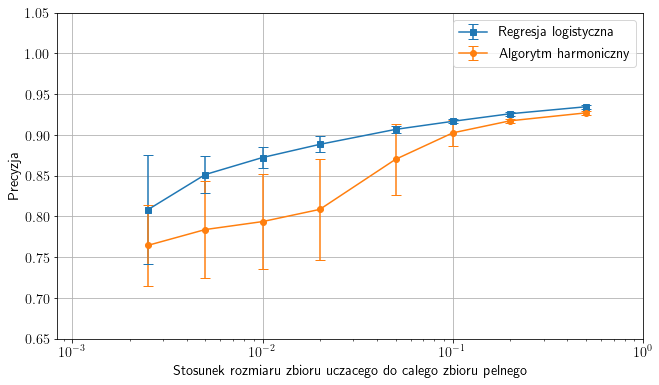
\includegraphics[width=0.95\linewidth]{img/results/wyniki-pelen.png}
	\caption{Wykres uzyskanej precyzji dla różnych rozmiarów zbioru uczącego, wykonane dla zbioru pełnego.}	\label{fig:wyniki-pelen}
\end{figure}
\par
Patrząc na wykres na rysunku \ref{fig:wyniki-pelen} w\,przypadku mniejszych zbiorów uczących widać wyraźną przewagę regresji liniowej. Używając jej, mając zaklasyfikowany nawet tylko 1\% danych, jesteśmy w\,stanie uzyskać precyzję w\,wysokości 87\%. Natomiast algorytm harmoniczny daje niższą precyzję w\,dodatku z\,ryzykiem odchylenia w\,zależności od dobranego zbioru. 
\par
Uzyskane wyniki robią wrażenie biorąc pod uwagę, że w\,omawianym tu przypadku, dzięki zastosowaniu regresji logistycznej z\,wiedzy na temat 150 postów jesteśmy w\,stanie z\,taką precyzją podać do jakich klas może należeć pozostałe ponad 15 tysięcy postów. Nie jest to jednak wynik, który można by zastosować w\,realnym systemie automatycznej klasyfikacji postów, chcąc aby był możliwie dokładny i\,pozbawiony błędów. 



\newpage
\par
\textbf{Zbiór intersekcji} 
\par
W przypadku zbioru intersekcji dla obu algorytmów otrzymano wyniki trochę gorsze od zbioru pełnego. Nie jest to zaskakujące odkrycie, ponieważ liczba postów nie różni się dużo od liczby postów w\,zbiorze pełnym, jest bowiem tylko 25 \% mniejsza, natomiast znacznie się różni liczba cech tych postów. W\,zbiorze zawarto połowę mniej udostępnień wykonaną przez mniej niż jedną czwartą użytkowników niż w\,zbiorze pełnym. Co więcej należy pamiętać, że prawie połowa tych osób wykonała tylko jedno udostępnienie co omawiano we wcześniejszym rozdziale. 
\par
Z tego też powodu precyzję większą niż 90\% uzyskano jedynie dla zbiorów uczących posiadających przynajmniej 20\% postów z\,całego zbioru, i\,to tylko dla regresji logistycznej. Ta metoda również dla zbioru intersekcji okazała się dawać lepsze wyniki. 
\par
Na wykresie jest widoczne, że dla zbioru intersekcji lepsze wyniki są uzyskiwane dla regresji logistycznej niż dla algorytmu harmonicznego dla każdej wielkości zbioru uczącego. Szczególna różnica występuje dla zbiorów poniżej 1000 postów. To zjawisko można wytłumaczyć faktem, że aby w\,algorytmie harmonicznym użytkownik był ściśle zakwalifikowany do jednej z\,etykiet musi posiadać dwa razy więcej udostępnień w\,jednej z\,klas niż w\,drugiej. Przy mniejszym zbiorze uczącym może się zdarzyć, że podając znane etykiety tylko części postów, wiedza może być błędnie propagowana. Prostym przykładem wyjaśniającym taki przypadek jest użytkownik, który posiada tylko dwa udostępnienia, po jednym w\,każdej klasie. Jeśli w\,zbiorze uczącym znajdzie się tylko jeden z\,tych postów użytkownik zostanie zakwalifikowany jako preferujący tą klasę, gdy w\,rzeczywistości tak nie jest. W\,ten sposób błędna informacja zostanie rozpropagowana w\,grafie. Teorię tą potwierdza wysokie odchylenie standardowe pokazujące różnice jakie są uzyskiwane między kolejnymi iteracjami algorytmu z\,różnym zbiorem danych uczących. 

\begin{table}[!h]
\centering
\caption{Wyniki badań klasyfikacji dla zbioru intersekcji - porównanie precyzji dla różnego stosunku zbioru uczącego do całego zbioru.} \label{tab:precyzjazbiorintersekcji}
\begin{tabular}{|L{3cm}|R{2,5cm}|R{2,5cm}|R{2,5cm}|R{2,5cm}|} 
\hline
~ & \multicolumn{2}{l|}{Regresja logistyczna} & \multicolumn{2}{l|}{Algorytm harmoniczny} \\ 
\hline
Stosunek zbioru uczącego do całego zbioru & Precyzja & Odchylenie standardowe & Precyzja & Odchylenie standardowe \\ 
\hline
0.5 & 0.911 & 0.003 & 0.887 & 0.004 \\ 
\hline
0.2 & 0.901 & 0.003 & 0.875 & 0.004 \\ 
\hline
0.1 & 0.893 & 0.004 & 0.856 & 0.019 \\ 
\hline
0.05 & 0.882 & 0.004 & 0.802 & 0.083 \\ 
\hline
0.02 & 0.865 & 0.010 & 0.756 & 0.109 \\ 
\hline
0.01 & 0.842 & 0.018 & 0.666 & 0.133 \\ 
\hline
0.005 & 0.816 & 0.023 & 0.634 & 0.137 \\ 
\hline
0.0025 & 0.761 & 0.057 & 0.586 & 0.138 \\
\hline
\end{tabular}
\end{table}


\par
Dla zbioru uczącego zawierającego tylko 1\% danych całego zbioru wyniki algorytmu harmonicznego są już niewiele wyższe od losowego zgadywania. W\,przypadku regresji logistycznej nawet przy tak małym zbiorze uczącym w\,stosunku do całości testowanych danych precyzja wynosi 84\% z\,odchyleniem 0,01 pomiędzy przypadkami. Jest to wynik nadal zaskakująco zadowalającym biorąc pod uwagę, że oznacza to 120 postów w\,zbiorze uczącym i\,prawie 12 tysięcy w\,zbiorze testowym.

\begin{figure}[!h]
	
	\centering 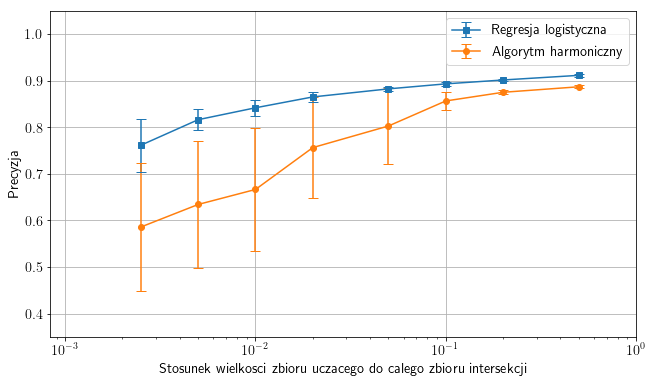
\includegraphics[width=0.95\linewidth]{img/results/wyniki-intersekcja.png}
	\caption{Wykres uzyskanej precyzji dla różnych rozmiarów zbioru uczącego, wykonane dla zbioru intersekcji.}\label{fig:wyniki-intersekcja}
\end{figure}

\subsubsection{Transmisja wiedzy w\,modelu}
W ostatnim badaniu chciano sprawdzić, jak sprawdzają się powyżej omawiane algorytmy w\,propagowaniu wiedzy o\,możliwej klasyfikacji postów pochodzących z\,różnych kont. W\,tym celu odrzucano do zbioru testowego wszystkie posty należące do wybranej liczby określonych kont. Wyniki nie okazały się być jednak obiecujące. Regresja logistyczna uzyskała średnie wyniki niewiele wyższe od losowego zgadywania. 
\par
Dla badania przy odrzuceniu jednego konta do zbioru testowego średnia precyzja regresji logistycznej dla zbioru pełnego wynosiła 0.70 oraz dla zbioru intersekcji 0,68, dla obu przypadków odchylenie wynosi 0,3 
Wyniki nie są wcale lepsze przy użyciu algorytmu harmonicznego wykorzystującego dane w\,postaci grafu. Średnie wyniki okazały się być równie niskie wynosząc 0,65 dla zbioru pełnego oraz bardzo niskie, wręcz błędne 0,3 dla zbioru intersekcji. W\,tym jednak przypadku odchylenie precyzji pomiędzy przypadkami jest ogromne sięgając 0,4 dla zbioru pełnego jak i\,dla zbioru intersekcji. 




\begin{table}[!h]
\centering
\caption{Wyniki badań transmisji wiedzy - porównanie precyzji dla dwóch typów badań, odrzucenie jednego konta lub połowy kont.} \label{tab:precyzjazbiorintersekcji}
\begin{tabular}{|L{2cm}|L{2cm}|R{1,8cm}|R{2,5cm}|R{1,8cm}|R{2,5cm}|} 
\hline
~ & ~  & \multicolumn{2}{l|}{Regresja logistyczna} & \multicolumn{2}{l|}{Algorytm harmoniczny} \\ 
\hline
Typ \mbox{badania} & Typ zbioru & Precyzja & Odchylenie standardowe & Precyzja & Odchylenie standardowe \\ 
\hline
\multirow{2}{2cm}{Odrzucenie jednego konta} & Zbiór pełny & 0,700 & 0,372 & 0,658 & 0,403 \\ 
\cline{2-6}
 & Zbiór \mbox{intersekcji} & 0,683 & 0,355 & 0,300 & 0,472 \\ 
\hline
\multirow{2}{2cm}{Odrzucenie połowy kont} & Zbiór pełny & 0,645 & 0.098 & 0,647 & 0,125 \\ 
\cline{2-6}
 & Zbiór \mbox{intersekcji} & 0,570 & 0,097 & 0,504 & 0,124 \\
\hline
\end{tabular}
\end{table}

\par
Przyglądając się więc, dokładniej poszczególnym wynikom obu algorytmów można zauważyć, że dla niektórych przypadków precyzja klasyfikacji była bardzo wysoka sięgając nawet 100 procent, ale dla niektórych wynosiła praktycznie zero. Oznacza to, że w\,przypadku postów pochodzących z\,niektórych stron albo nie było istniejącego połączenia z\,zaklasyfikowanymi danymi albo też połączenia te wskazywały na inną klasę niż zostało to pierwotnie założone. W\,praktyce, w\,omawianym przypadku, oznacza to, że albo niektóre konta nie mają wspólnych udostępniających użytkowników z\,pozostałymi. Albo ich udostępniający głównie dokonują interakcji z\,postami publikowanymi przez strony zakwalifikowane w\,tej pracy do przeciwnej klasy. Taka sytuacja może w\,szczególności występować w\,zbiorze intersekcji, gdzie udostępnień jest znacznie mniej. 
\par

Jak można się było spodziewać, dokonując badań przy odrzuceniu postów z\,połowy kont do zbioru testującego nie otrzymano lepszych wyników. Jedynie odchylenie zmalało jest to jednak zasługa zmieszania różnego rodzaju kont, które w\,rezultacie dały podobnie losowe wyniki. 

\subsection{Wnioski z badań}
Na podstawie wykonanych badań można jasno określić, że najlepszym sposobem do klasyfikacji tego typu danych okazała się regresja logistyczna. Uzyskane dzięki niej wyniki przewyższały wyniki algorytmu harmonicznego zarówno dla zbioru pełnego jak i\,dla zbioru intersekcji. Dodatkowo zbadano, że przy zbiorze pełnym wystarczy, aby znano klasyfikację jedynie dziesięciu procent badanych postów, aby z\,precyzją 90\% określić klasy pozostałych postów. 
\par
	Niestety jednak okazało się, że żaden z\,powyższych algorytmów nie spełnia dobrze zadania transmisji wiedzy w\,modelu, jeśliby odrzucić posty opublikowane przez konkretne konta do zbioru testowego. Nie jest to jednak wina wybranych algorytmów, ale ułożenia danych. Dla niektórych z\,kont klasyfikacja ich postów była dokonywana z\,prawie 100\% precyzją. Średni wynik zaniżały jednak inne konta, które nie miały wystarczająco wspólnych udostępniających użytkowników. 
\par
Dodatkowo warto zaznaczyć, że wszystkie powyżej opisane badania były robione kilkakrotnie dla różnej liczby pobranych postów rozpoczynając od 8 tysięcy postów. Przy zwiększaniu ilości danych nie zauważono znacznej poprawy wyników klasyfikacji dla wszystkich przedziałów podziału zbioru na uczący i\,testowy. Dlatego pozostano przy tweetach pobranych z\,okresu 20 dni. Po przeprowadzonej analizie badań można zauważyć, że wysoka precyzja utrzymuje się nawet dla 10\% danych w\,zbiorze uczącym, czyli wystarczy około 1200-1500 postów w\,zależności od zbioru.

\newpage % Rozdziały zaczynamy od nowej strony.
\section{Podsumowanie}

                                        % Wygodnie jest trzymać każdy rozdział w osobnym pliku.
%\newpage % Rozdziały zaczynamy od nowej strony.
\section{De Finibus Bonorum et Malorum}
Tu dam moj tekst.  Lorem ipsum dolor sit this is thext \footnote{This is footnote.}.
\begin{align*}
    E & = mc^2 \\
    y & = ax^2 + bx + c
\end{align*}

\lipsum[3]

\begin{align}
\begin{bmatrix}
    1 & 0 & 0 \\
    0 & 2 & 0 \\
    0 & 0 & 3
\end{bmatrix} \cdot
\begin{bmatrix}
    4 \\ 5 \\ 6
\end{bmatrix} =
\begin{bmatrix}
    4 \\ 10 \\ 18
\end{bmatrix}
\end{align}

\lipsum[4] Lorem ipsum dolor sit amet, consectetur adipiscing elit, sed do eiusmod tempor incididunt ut labore et dolore magna aliqua \cite{szczypiorski2015}, \cite{duqu2011}, \cite{shs2015}, \cite{wozniak2018}, \cite{dcp19}.

\subsection{Critique of Pure Reason}
\kant[1]

\begin{table}[!h] \label{tab:tabela1} \centering
\caption{Przykładowa tabela.}
\begin{tabular} {| c | c | r |} \hline
    Kolumna 1 & Kolumna 2 & Liczba \\ \hline\hline
    cell1 & cell2 & 60 \\ \hline
    cell4 & cell5 & 43 \\ \hline
    cell7 & cell8 & 20,45 \\ \hline
    \multicolumn{2}{|r|}{Suma:} & 123,45 \\ \hline
\end{tabular}
\end{table}

\kant[2]

\begin{longtable}{| c | m{0.58\linewidth} | r | m{0.1\linewidth} |}
    \caption{Tabela wielostronicowa.} \\
    \hline
    Lp & \multicolumn{1}{c|}{Treść} & \multicolumn{1}{c|}{Kwota} & \multicolumn{1}{m{0.1\linewidth}|}{Wariant opłaty} \\ \hline\hline \endfirsthead

    \endfoot
    \hline \endlastfoot

    1 & Lorem ipsum dolor sit amet, consectetur adipiscing elit, sed do eiusmod tempor incididunt ut labore et dolore magna aliqua. & 111 111,11 zł & \multicolumn{1}{c|}{WAR1} \\ \hline
    2 & Lorem ipsum dolor sit amet, consectetur adipiscing elit, sed do eiusmod tempor incididunt ut labore et dolore magna aliqua. & 22 222,22 zł & \multicolumn{1}{c|}{WAR1} \\ \hline
    3 & Lorem ipsum dolor sit amet, consectetur adipiscing elit, sed do eiusmod tempor incididunt ut labore et dolore magna aliqua. & 33 333,33 zł & \multicolumn{1}{c|}{WAR1} \\ \hline
    4 & Lorem ipsum dolor sit amet, consectetur adipiscing elit, sed do eiusmod tempor incididunt ut labore et dolore magna aliqua. & 444 444,44 zł & \multicolumn{1}{c|}{WAR1} \\ \hline
    5 & Lorem ipsum dolor sit amet, consectetur adipiscing elit, sed do eiusmod tempor incididunt ut labore et dolore magna aliqua. & 55 555,55 zł & \multicolumn{1}{c|}{WAR1} \\ \hline
    6 & Lorem ipsum dolor sit amet, consectetur adipiscing elit, sed do eiusmod tempor incididunt ut labore et dolore magna aliqua. & 66 666,66 zł & \multicolumn{1}{c|}{WAR1} \\ \hline
    7 & Lorem ipsum dolor sit amet, consectetur adipiscing elit, sed do eiusmod tempor incididunt ut labore et dolore magna aliqua. & 777 777,77 zł & \multicolumn{1}{c|}{WAR1} \\ \hline
    8 & Lorem ipsum dolor sit amet, consectetur adipiscing elit, sed do eiusmod tempor incididunt ut labore et dolore magna aliqua. & 8 888,88 zł & \multicolumn{1}{c|}{WAR1} \\ \hline
    9 & Lorem ipsum dolor sit amet, consectetur adipiscing elit, sed do eiusmod tempor incididunt ut labore et dolore magna aliqua. & 999 999,99 zł & \multicolumn{1}{c|}{WAR1} \\ \hline
    10 & Lorem ipsum dolor sit amet, consectetur adipiscing elit, sed do eiusmod tempor incididunt ut labore et dolore magna aliqua. & 111 111,11 zł & \multicolumn{1}{c|}{WAR2} \\ \hline
    11 & Lorem ipsum dolor sit amet, consectetur adipiscing elit, sed do eiusmod tempor incididunt ut labore et dolore magna aliqua. & 22 222,22 zł & \multicolumn{1}{c|}{WAR2} \\ \hline
    12 & Lorem ipsum dolor sit amet, consectetur adipiscing elit, sed do eiusmod tempor incididunt ut labore et dolore magna aliqua. & 33 333,33 zł & \multicolumn{1}{c|}{WAR2} \\ \hline
    13 & Lorem ipsum dolor sit amet, consectetur adipiscing elit, sed do eiusmod tempor incididunt ut labore et dolore magna aliqua. & 444 444,44 zł & \multicolumn{1}{c|}{WAR2} \\ \hline
    14 & Lorem ipsum dolor sit amet, consectetur adipiscing elit, sed do eiusmod tempor incididunt ut labore et dolore magna aliqua. & 55 555,55 zł & \multicolumn{1}{c|}{WAR2} \\ \hline
    15 & Lorem ipsum dolor sit amet, consectetur adipiscing elit, sed do eiusmod tempor incididunt ut labore et dolore magna aliqua. & 66 666,66 zł & \multicolumn{1}{c|}{WAR2} \\ \hline
    & \multicolumn{1}{r|}{\textbf{Suma:}} & \textbf{7 777 777,77 zł} &
    \label{table:koszty}
\end{longtable}
\kant[4]

\subsection{Categorical Imperative}
\subsubsection{Deontological Ethics}
As any dedicated reader can clearly see, the Ideal of practical reason is a representation of, as far as I know, the things in themselves; as I have shown elsewhere, the phenomena should only be used as a canon for our understanding:
% Parametr label ustawia symbol, a leftmargin - wielkość wcięcia.
% Domyślny układ to [---] bez wcięcia, bo tak pan Marcin Woliński powiedział;
% ale ja nie polecam. // AB
\begin{itemize}
    \item Item 1:
    \begin{itemize}[label=---]
        \item item 1.1;
        \item item 1.2;
        \item item 1.3;
    \end{itemize}
    \item Item 2;
    \item Item 3;
    \item Item 4.
\end{itemize}
\kant[2]

\subsubsection{Consequentialism -- the Ideal of practical reason}
\kant[3]
\begin{enumerate}
    \item Item 1:
    \begin{enumerate}
        \item item 1.1;
        \item item 1.2:
        \begin{enumerate}
            \item item 1.2.1;
            \item item 1.2.2;
        \end{enumerate}
        \item item 1.3;
    \end{enumerate}
    \item Item 2;
    \item Item 3;
    \item Item 4.
\end{enumerate}

\kant[9]

\subsection{G\"odel's ontological proof}
\kant[9] Lorem ipsum dolor sit amet, consectetur adipiscing elit, sed do eiusmod tempor incididunt ut labore et dolore magna aliqua \cite{benzmuller2014}, \cite{goedel95}, \cite{wang97}, \cite{koons2005}.
\begin{assumption} \label{ass:1}
    $ [\![ \ \phi \ ]\!] \Longrightarrow [\![ \ P(\phi); \neg P(\phi) \ ]\!]$
\end{assumption}
\begin{axiom}[Dualność] \label{axiom:1}
    $\neg P(\phi) \Leftrightarrow P(\neg \phi)$, równoważnie $P(\phi) \Leftrightarrow \neg P(\neg \phi)$
\end{axiom}
\begin{axiom}[Całkowitość] \label{axiom:2}
    $ \left( P(\phi) \wedge \forall x: \phi(x) \Rightarrow \psi(x) \right) \Rightarrow P(\psi) $
\end{axiom}
\begin{axiom}[Absolutność] \label{axiom:3}
    $ P(\phi) \Rightarrow \Box P(\phi) $
\end{axiom}
\begin{definition} \label{def:1}
    $ G(x) \Leftrightarrow \forall \phi: \left( P(\phi) \Rightarrow \phi(x) \right) $
\end{definition}
\begin{definition} \label{def:2}
    $ \phi \ ess \ x \Leftrightarrow \phi(x) \wedge \forall \psi \left( \psi(x) \Rightarrow \Box \forall y \left( \phi(y) \Rightarrow \psi(y) \right) \right)  $
\end{definition}
\begin{axiom} \label{axiom:4}
    P(G)
\end{axiom}
\begin{lemma} \label{lemma:1}
    $ P(\phi) \Rightarrow \Diamond \exists x : \phi(x) $
\end{lemma}
\begin{proof}
    Dowód pomijamy, bo jest trywialny :)
\end{proof}
\begin{lemma} \label{lemma:2}
    $ \Diamond \exists x : G(x) $
\end{lemma}
\begin{proof}
    Natychmiastowy wniosek z aksjomatu \ref{axiom:4} i lematu \ref{lemma:1}.
\end{proof}
\begin{lemma} \label{lemma:3}
    $ G(x) \Rightarrow G \ ess \ x $
\end{lemma}
\begin{proof}
    Poprzez podstawienie do definicji \ref{def:2}.
\end{proof}
\begin{definition} \label{def:3}
    $ E(x) \Leftrightarrow \forall \phi \left( \phi \ ess \ x \Rightarrow \Box\ \exists x: \phi(x) \right) $
\end{definition}
\begin{axiom} \label{axiom:5}
    P(E)
\end{axiom}
\begin{theorem}
    $ \Box\ \exists x : G(x) $
\end{theorem}
\begin{proof}
    Na podstawie definicji \ref{def:1}, lematu \ref{lemma:3} i aksjomatu \ref{axiom:5}.
\end{proof}    % Umożliwia to również łatwą migrację do nowej wersji szablonu:
%\newpage % Rozdziały zaczynamy od nowej strony.
\section{Code listings}

\lipsum[10]
% \addmargin pozwala na wcięcie kodu od lewej (tutaj: 6mm).
% Wcięcie pomaga ustawić kod tak, 
% aby numery linii nie były za bardzo na lewo. 
% Druga liczba oznacza wcięcie od prawej. 
\begin{addmargin}[6mm]{0mm}
\begin{lstlisting}[
    language=HTML,
    numbers=left,
    firstnumber=1,
    caption={\emph{Hello world} w HTML},
    aboveskip=0pt
]
<html>
  <head>
    <title>Hello world!</title>
  </head>
  <body>
    Hello world!
  </body>
</html>
\end{lstlisting}
\end{addmargin}

\lipsum[11]
% Dla dłuższych numerów linii
% potrzebne jest większe wcięcie.
\begin{addmargin}[10mm]{0mm}
\begin{lstlisting}[
    language=C++,
    numbers=left,
    firstnumber=147,
    caption={Generowanie sekwencji Collatza w języku C++},
    aboveskip=0pt
]
class Collatz {
  private:
    unsigned current_val_;
    void update_val() {
        if( current_val_ % 2 == 0 )
            current_val_ /= 2;
        else
            current_val_ = current_val_ * 3 + 1;
    }

  public:
    explicit Collatz(unsigned initial_value) : 
        current_val_(initial_value) {}
    void print_sequence() {
        unsigned i = 1;
        while( current_val_ > 1 ) {
            std::cout
                << "val " << i << " = " << current_val_
                << std::endl;
            update_val(); ++i;
        }
    }
};

int main() {
  // prints Collatz seqence, starting from 194375
  Collatz seq(194375);
  seq.print_sequence();
  return 0;
}
\end{lstlisting}
\end{addmargin}

\lipsum[12]
 % wystarczy podmienić swoje pliki main.tex i eiti-thesis.cls
                            % na nowe wersje, a cały tekst pracy pozostaje nienaruszony.

% \newpage % Rozdziały zaczynamy od nowej strony
% \section{Summatio}          % Można też pisać rozdziały w jednym pliku.
% \lipsum[5-10]

%--------------------------------------------
% Literatura
%--------------------------------------------
\cleardoublepage % Zaczynamy od nieparzystej strony
\printbibliography

%--------------------------------------------
% Spisy (opcjonalne)
%--------------------------------------------
\newpage
\pagestyle{plain}

% Wykaz symboli i skrótów.
% Pamiętaj, żeby posortować symbole alfabetycznie
% we własnym zakresie. Ponieważ mało kto używa takiego wykazu,
% uznałem, że robienie automatycznie sortowanej listy
% na poziomie LaTeXa to za duży overkill.
% Makro \acronymlist generuje właściwy tytuł sekcji,
% w zależności od języka.
% Makro \acronym dodaje skrót/symbol do listy,
% zapewniając podstawowe formatowanie.
% //AB
% \vspace{0.8cm}
% \acronymlist
% \acronym{EiTI}{Wydział Elektroniki i Technik Informacyjnych}
% \acronym{PW}{Politechnika Warszawska}
% \acronym{WEIRD}{ang. \emph{Western, Educated, Industrialized, Rich and Democratic}}

\listoffigurestoc     % Spis rysunków.
\vspace{1cm}          % vertical space
\listoftablestoc      % Spis tabel.
\vspace{1cm}          % vertical space
% \listofappendicestoc  % Spis załączników

% % Załączniki
% \newpage
% \appendix{Nazwa załącznika 1}
% \lipsum[1-8]

% \newpage
% \appendix{Nazwa załącznika 2}
% \lipsum[1-4]

% Używając powyższych spisów jako szablonu,
% możesz tu dodać swój własny wykaz bądź listę,
% np. spis algorytmów.

\end{document} % Dobranoc.
